\documentclass[11pt,a4paper]{article}
\usepackage[margin=23mm,headheight=15pt,footskip=12mm]{geometry}
\usepackage{fontspec}
\IfFileExists{fonts/NotoSansCJKkr-Regular.otf}{
\setmainfont{NotoSansCJKkr-Regular.otf}[Path=fonts/,BoldFont=NotoSansCJKkr-Bold.otf,ItalicFont=NotoSansCJKkr-Regular.otf,ItalicFeatures={FakeSlant=0.12}]
\setmonofont{DejaVuSansMono.ttf}[Path=fonts/,Scale=0.75]
}{
\setmainfont{Noto Sans CJK KR}
\setmonofont{DejaVu Sans Mono}[Scale=0.75]
}
\XeTeXlinebreaklocale "ko"
\XeTeXlinebreakskip=0pt plus 0.1em
\usepackage{amsmath,amssymb,mathtools,mathrsfs,graphicx,booktabs,longtable,array}
\usepackage[table,dvipsnames]{xcolor}
\usepackage{enumitem,fancyhdr,titlesec}
\usepackage[unicode,colorlinks=true,linkcolor=MidnightBlue,urlcolor=MidnightBlue,citecolor=MidnightBlue]{hyperref}
\usepackage{xurl,microtype}
\providecommand{\tightlist}{\setlength{\itemsep}{2pt}\setlength{\parskip}{0pt}}
\providecommand{\pandocbounded}[1]{#1}
\setlength{\parindent}{0pt}
\setlength{\parskip}{5pt}
\setlength{\emergencystretch}{3em}
\setlength{\LTpre}{6pt}
\setlength{\LTpost}{8pt}
\setlist{leftmargin=1.6em,itemsep=2pt,topsep=4pt}
\renewcommand{\arraystretch}{1.14}
\linespread{1.08}
\pagestyle{fancy}\fancyhf{}
\fancyhead[L]{\small BASS\_CR · 실제 kernel과 온도 의존 cutoff}
\fancyhead[R]{\small 이론 연구 루프}
\fancyfoot[C]{\thepage}
\titleformat{\section}{\Large\bfseries\color{MidnightBlue}}{\thesection}{.7em}{}
\titleformat{\subsection}{\large\bfseries}{\thesubsection}{.7em}{}
\titleformat{\subsubsection}{\normalsize\bfseries}{\thesubsubsection}{.7em}{}
\setcounter{tocdepth}{1}
\renewcommand{\contentsname}{차례}
\hypersetup{pdftitle={BASS_CR: actual kernel events and temperature-dependent cutoff},
pdfauthor={BASS_CR research record},pdfsubject={CR-THEORY-KERNEL-CUTOFF-20261013}}
\begin{document}
\begin{titlepage}
{\color{MidnightBlue}\large BASS\_CR 연구노트\par}
\vspace{16mm}
{\Huge\bfseries 실제 충돌 kernel과\\[3mm]온도 의존 cutoff의 결합\par}
\vspace{8mm}
{\Large 양의 사건 분해 · 유한 열적 재분류 · 공변 에너지 장부\par}
\vspace{12mm}
{\large 다음 이론 연구 루프\par}
\vspace{4mm}
{2026년 10월 13일 (KST)\par}
\vspace{12mm}
\begin{minipage}{.96\textwidth}
\large
저장된 9600개 에너지 격자와 HI·HeI collision kernel을
보존 사건 열에 연결하고, 온도에 따라 움직이는 cutoff의
유한 count·energy 분할과 양의 해를 구성했다.
연속 spectrum의 오차 certificate, 원자 branch의 유한 알고리즘,
Wolfram·xAct 검산 및 독립 검토를 함께 제공한다.
\end{minipage}
\vfill
\begin{tabular}{@{}ll@{}}
연구 단위 & CR-THEORY-KERNEL-CUTOFF-20261013\\
구성 & 실제 kernel · 유한 cutoff · coupled feedback\\
검산 & 실제 사건 17개 · Wolfram/xAct 28개 그룹\\
도구 & SciSpace · Exa · Wolfram Language · xAct\\
내용 & 전체 유도 · 정확한 사례 · 구현 · DAG · 원출력\\
\end{tabular}
\end{titlepage}
\tableofcontents
\clearpage
\hypertarget{uxc774uxbc88-uxb8e8uxd504uxc758-uxacb0uxacfc}{%
\section{이번 루프의 결과}\label{uxc774uxbc88-uxb8e8uxd504uxc758-uxacb0uxacfc}}

실제 저장된 9600개 에너지 격자와 HI·HeI collision kernel을, 입자수·전하·에너지를 함께 보존하는 양의 사건 분해에 연결했다. 이어 \(E_c(T)=\chi k_BT\)로 움직이는 cutoff를 같은 원시 입자 inventory에서 재분류하는 유한 map을 구성하고, 온도 방정식의 해·오차·feedback 조건을 도출했다. 원자 격자에는 유한 branch 알고리즘을, 연속 spectrum에는 검증 가능한 root certificate를 제공한다.

이번 연구 단위는 \textbf{CR-THEORY-KERNEL-CUTOFF-20261013}이다. 직전 승인된 FB1--FB7과 그 DAG에서 열려 있던 실제 kernel 사건 adapter 및 온도 의존 cutoff 두 노드를 수행했다. 이전의 공통 사건량, 양의 재고 제한식, thermal/all-free 변환과 이동 경계 장부는 근거 identity를 유지하여 재사용했다. 이번에 새로 계산한 대상과 실행 결과는 아래에 한 번에 정리했다.

\hypertarget{uxd575uxc2ec-uxacb0uxb860}{%
\subsection{핵심 결론}\label{uxd575uxc2ec-uxacb0uxb860}}

\begin{enumerate}
\def\labelenumi{\arabic{enumi}.}
\tightlist
\item
  \textbf{실제 daughter 분배를 보존하는 사건 step.} 같은 parent와 target species에 속한 모든 sharing 사건의 donor가 같음을 실제 격자 간격과 문턱 에너지로 증명했다. 이에 따라 양수성을 보장하는 capacity 제한은 같은 family의 전체 사건량을 조정하며 원래 daughter sharing probability를 유지한다.
\item
  \textbf{온도에 따라 움직이는 cutoff의 유한 해.} 전체 count와 kinetic energy를 고정하고 실제 이동 band의 0차·1차 모멘트를 다시 평가한다. 이 map에서 EOS를 풀면 연속 분포의 유효 열용량, 양의 유일근 조건, 잔차로부터의 온도 오차 한계가 함께 나온다.
\item
  \textbf{저장된 원자 격자에 맞는 구성.} Node별 입자수를 그대로 유지하면서 열적 prefix의 가능한 해를 유한하게 열거한다. \(\chi\ge3/2\)에서는 양의 base에서 해를 유한 단계로 구성할 수 있고, 고정 spectrum에 대한 가열·냉각 continuation은 기존 branch를 이어 간다.
\item
  \textbf{공변 경계식과 coupled feedback.} 수 전류와 총 4-momentum source의 rest-mass subtraction을 연결했다. 사건의 에너지·열적 입자수 증분으로 전체 온도·밀도·조성 map의 수축상계와 inner/outer 오차식을 얻었다.
\end{enumerate}

독립 판정: \textbf{PROMOTE\_SCOPED}. 주장 KC1--KC7의 정확한 범위와 근거는 \texttt{CLAIMS.json}, 전제는 \texttt{CONTRACT.json}, 독립 검토의 동결 대상은 \nolinkurl{review/CANDIDATE_MANIFEST.json}에 있다. 이 보고서의 ``완료''는 그 전제 아래의 이론 구성과 reference 구현에 관한 판정이다.

\hypertarget{uxd604uxc7ac-uxac00uxc815uxacfc-uxadfcuxac70}{%
\subsection{현재 가정과 근거}\label{uxd604uxc7ac-uxac00uxc815uxacfc-uxadfcuxac70}}

\begin{longtable}[]{@{}
  >{\raggedright\arraybackslash}p{(\columnwidth - 4\tabcolsep) * \real{0.3333}}
  >{\raggedright\arraybackslash}p{(\columnwidth - 4\tabcolsep) * \real{0.3333}}
  >{\raggedright\arraybackslash}p{(\columnwidth - 4\tabcolsep) * \real{0.3333}}@{}}
\toprule\noalign{}
\begin{minipage}[b]{\linewidth}\raggedright
대상
\end{minipage} & \begin{minipage}[b]{\linewidth}\raggedright
이번에 고정한 내용
\end{minipage} & \begin{minipage}[b]{\linewidth}\raggedright
근거와 역할
\end{minipage} \\
\midrule\noalign{}
\endhead
\bottomrule\noalign{}
\endlastfoot
기하와 단위 & \((-,+,+,+)\); \(c,k_B,\hbar\) 유지; 상태 에너지 J, 원자 입력 eV; proper time & CV.1--10, KA.1--4 \\
실제 입력 & PHYS02C full BED HI·HeI, PHYS02B projection·stopping·CCC; 저장된 9600 nodes & 기준 commit의 11개 원본 파일과 실제 NPZ bytes \\
사건과 재고 & 한 사건의 모든 증분에 같은 extent; 초기 active mask와 초기 donor support 고정 & KA.12--29 및 기존 FP.7--24 \\
Coulomb bath & \(n_e=N_{e,\mathrm{th}}/V\); 양의 Coulomb log와 cold-target 범위 & KA.19--24 \\
열적 EOS & \(U=c_vNT\), \(c_v=3k_B/2\); \(N\)은 핵종과 thermal electrons의 합 & TCF.2--13 \\
유한 분할 & 하나의 root solve에서 전체 count·energy·spectrum을 고정; lower trace 보존 & TCF.2--10 \\
연속 root & root bracket과 \(C_{\rm eff}\ge m>0\) & TCF.13--24 \\
원자 root & equality는 thermal 소유; finite branch 열거; 존재 scan에는 \(\chi\ge3/2\) & TCF.36--46 \\
결합 feedback & descriptor self-map, uniform bracket, \(q<1\); 연속 표현의 기저는 trial과 독립 & CP.1--15 \\
\end{longtable}

원본 격자의 첫 node는 0.10309375000000001 eV, 중간 연결 node는 10 eV, 마지막 node는 900 eV다. Source lower absorber는 0.1 eV다. 실제 NPZ와 그 안의 energy array를 읽었으며, grid raw SHA256은 \nolinkurl{6a76d3539115003b046a5861baca89b0a4ff966564627e04d9f6e8bc86be8292}이다. 기존 spectrum을 다시 계산하거나 전체 generator를 새로 만들지 않았다.

\hypertarget{uxc2e4uxc81c-kerneluxc744-uxbcf4uxc874-uxc0acuxac74uxc73cuxb85c-uxc5f0uxacb0uxd55c-uxacb0uxacfc}{%
\section{실제 kernel을 보존 사건으로 연결한 결과}\label{uxc2e4uxc81c-kerneluxc744-uxbcf4uxc874-uxc0acuxac74uxc73cuxb85c-uxc5f0uxacb0uxd55c-uxacb0uxacfc}}

\hypertarget{uxb450-uxb538uxc744-uxd558uxb098uxc758-uxc0acuxac74uxc73cuxb85c-uxbb36uxb294-uxc774uxc720}{%
\subsection{두 딸을 하나의 사건으로 묶는 이유}\label{uxb450-uxb538uxc744-uxd558uxb098uxc758-uxc0acuxac74uxc73cuxb85c-uxbb36uxb294-uxc774uxc720}}

Parent energy \(E_j\), ionization threshold \(B_a\), 실제 sharing point \(w_\ell\)에 대해 두 daughter energy는

\[
w_1=w_\ell,\qquad w_2=E_j-B_a-w_\ell
\]

이다. 각 daughter를 양의 barycentric weights로 grid와 lower absorber에 투영한다. 한 daughter의 active weights \(b_i\), 흡수 count \(n_B\), 실제 흡수 energy \(u_B\)는

\[
\sum_i b_i+n_B=1,\qquad \sum_iE_i b_i+u_B=w
\]

를 만족한다. 두 daughter를 더하고 parent 하나를 빼면 자유전자 수는 1 증가한다. 같은 사건에서 neutral 하나가 ion 하나로 바뀌므로 전하가 보존되고, threshold를 chemical energy로 넣으면 총 에너지도 보존된다. 실제 subcut absorption과 첫 grid cell의 ghost fraction은 별도 출력으로 남긴다.

원래 에너지 좌표의 discrete generator와 이 count-coordinate 사건 합의 대응도 직접 확인했다. \texttt{heat}, \texttt{cutoff\_energy}, \texttt{binding}, excitation energy 및 겹치는 observer를 각각 물리 장부와 대응시켜 같은 에너지를 두 번 더하지 않도록 했다. 전체 과정은 KA.5--18에 있다.

\hypertarget{uxac19uxc740-familyuxc758-daughter-uxbd84uxd3ecuxb97c-uxc720uxc9c0uxd558uxb294-uxac15uxd654-uxacb0uxacfc}{%
\subsection{같은 family의 daughter 분포를 유지하는 강화 결과}\label{uxac19uxc740-familyuxc758-daughter-uxbd84uxd3ecuxb97c-uxc720uxc9c0uxd558uxb294-uxac15uxd654-uxacb0uxacfc}}

실제 저장 격자의 최대 간격은 0.6325633326908928 eV이고, 최소 ion binding 13.6057 eV와 최소 adopted excitation cost 10.20435 eV보다 작다. 따라서 ion daughter나 excitation daughter의 투영은 parent node로 되돌아오지 않는다.

같은 \((j,a)\)에 속한 ionization 사건은 모두 동일한 donor \(\{A_j,X_a\}\)를 가지며 소비 계수도 1이다. 공유 재고로 만든 분모 \(1+h d_{ja}\)는 sharing index \(\ell\)에 독립이어서

\[
\boxed{\xi_{ja\ell}=p_{ja\ell}\,\Xi_{ja},\qquad
\Xi_{ja}=\frac{h\,m_j^nA_j^nv_j\sigma_a(E_j)X_a(z)/V}{1+h d_{ja}}.}
\]

이 성립한다. 같은 family 안에서 원래 \(p_{ja\ell}\)가 유지되는 결과다. 서로 다른 target species나 parent의 총 사건량은 각자의 경쟁하는 재고를 반영하여 달라질 수 있다. 이 일반성은 KA.29의 격자 간격 증명에 있고, 실제 세 sharing points의 exact ratio는 구현 연결을 확인한다.

\hypertarget{uxc2e4uxc81c-rate-feedbackuxc758-uxc704uxce58}{%
\subsection{실제 rate feedback의 위치}\label{uxc2e4uxc81c-rate-feedbackuxc758-uxc704uxce58}}

Fixed-energy atomic coefficient에는 직접적인 온도 인자가 없다. Trial neutral count가 atomic rate에 선형으로 들어가고, stopping은 thermal electron density를 통해 변한다. 기존 stopping prescription을 같은 에너지에서 이어 쓰면

\[
L_j(n)=L_j(n_0)-\frac12\log\frac n{n_0},\qquad b_j(n)=\alpha_jnL_j(n),
\]

\[
b_j'(n)=\alpha_j\left(L_j(n)-\frac12\right),\qquad
b_j''(n)=-\frac{\alpha_j}{2n}.
\]

양의 밀도 구간 양끝에서 \(|b_j'|\) 상계를 계산할 수 있다. Cutoff가 thermal ownership을 바꾸면 \(N_{e,\rm th}\)가 바뀌므로 이 식이 온도와 stopping의 간접 feedback을 연결한다. EOS에 넣는 총 thermal count에는 핵종도 포함되지만, screening 밀도에는 thermal electrons만 넣는다.

\hypertarget{uxc628uxb3c4-uxc758uxc874-cutoffuxb97c-uxc720uxd55c-uxb2e8uxacc4uxb85c-uxb2ebuxc740-uxacb0uxacfc}{%
\section{온도 의존 cutoff를 유한 단계로 닫은 결과}\label{uxc628uxb3c4-uxc758uxc874-cutoffuxb97c-uxc720uxd55c-uxb2e8uxacc4uxb85c-uxb2ebuxc740-uxacb0uxacfc}}

\hypertarget{uxac19uxc740-uxc804uxccb4-inventoryuxc5d0uxc11c-candidateuxb97c-uxacc4uxc0b0uxd55cuxb2e4}{%
\subsection{같은 전체 inventory에서 candidate를 계산한다}\label{uxac19uxc740-uxc804uxccb4-inventoryuxc5d0uxc11c-candidateuxb97c-uxacc4uxc0b0uxd55cuxb2e4}}

한 solve 동안 전체 count \(\mathscr C\), kinetic energy \(\mathscr E\), retained electron measure \(\mu\)를 고정한다. 아직 분해하지 않은 thermal base는

\[
N_B=\mathscr C-\int d\mu\ge N_{\rm nuc}>0,\qquad
U_B=\mathscr E-\int W\,d\mu\ge0
\]

를 만족한다. 경계 equality를 thermal 쪽에 배정하면

\[
\boxed{N(T)=\mathscr C-\mu((E_c(T),\infty)),\qquad
U(T)=\mathscr E-\int_{(E_c(T),\infty)}W\,d\mu.}
\]

이 계산은 모든 candidate에서 count와 kinetic energy를 정확히 보존한다. 낮은 에너지 전자를 이미 thermal로 합쳤더라도 그 원자 inventory를 retained measure에 남기면 cutoff를 낮출 때 회수할 수 있다. 이때 기존 thermal 총량에서 retained lower atoms를 먼저 빼서 \(N_B,U_B\)를 정의한다.

유한 이동의 에너지는 이동한 band의 1차 모멘트다. 따라서 일반적으로 \(\Delta U\ne E_c(T)\Delta N\)이다. 각 수치 반복은 같은 reference에서 새 candidate를 계산하며, 이전 반복에 다시 같은 이동량을 더하지 않는다.

\hypertarget{uxc720uxd6a8-uxc5f4uxc6a9uxb7c9uxacfc-uxc628uxb3c4-uxc624uxcc28}{%
\subsection{유효 열용량과 온도 오차}\label{uxc720uxd6a8-uxc5f4uxc6a9uxb7c9uxacfc-uxc628uxb3c4-uxc624uxcc28}}

연속 밀도 \(d\mu=\rho(W)dW\)에서

\[
F(T)=c_vTN(T)-U(T),\qquad E_c(T)=\chi k_BT
\]

를 미분하면

\[
\boxed{C_{\rm eff}=F_T=c_vN-\chi k_B(E_c-c_vT)\rho(E_c).}
\]

이 계수 자체는 기존 이동 경계 결과와 일치한다. 이번에는 유한 EOS map의 실제 미분으로 회복하고, root와 오차의 계산에 사용했다. \(\chi>3/2\)이면 경계의 편입 효과가 이 계수를 낮출 수 있다. 양의 \(N\)만으로 \(C_{\rm eff}>0\)를 대신할 수는 없다.

구간 \(I=[T_-,T_+]\)에서 \(F(T_-)\le0\le F(T_+)\)와 \(C_{\rm eff}\ge m>0\)를 확인하면 양의 유일근이 존재하며

\[
\boxed{|T-T^\star|\le\frac{|F(T)|}{m}}
\]

을 얻는다. 이번 finite box reference는 density knot 사이의 slope를 정확히 계산하여 \(m\)을 검증한다. 이분법의 bracket 오차와 이 잔차 bound 중 더 작은 값을 certificate로 반환한다. 물리 spectrum과 재구성 spectrum이 다르면 cutoff bracket의 tail count·energy 오차를 TCF.23--24로 추가한다.

\hypertarget{uxc815uxd655uxd55c-uxac00uxc5f4uxb0c9uxac01-uxc0acuxb840}{%
\subsection{정확한 가열·냉각 사례}\label{uxc815uxd655uxd55c-uxac00uxc5f4uxb0c9uxac01-uxc0acuxb840}}

\(\tau=T/T_*\), \(\epsilon=W/(k_BT_*)\)로 정규화하고, \(\chi=4\), \(dN/d\epsilon=\tfrac14\mathbf1_{[3,6]}\)를 택했다. 같은 전체 inventory에서 얻는 식은

\[
N(\tau)=1+\tau,\quad u(\tau)=1+\delta+2\tau^2,\quad
f(\tau)=\frac32\tau-\frac12\tau^2-1-\delta.
\]

\([3/4,5/4]\)에서 \(f'\ge1/4\)이고, \(-5/32\le\delta\le3/32\)이면 root가 존재한다. Picard map도 이 구간을 보존하며 그 미분은 \(233/243\) 이하이다.

\begin{longtable}[]{@{}
  >{\raggedright\arraybackslash}p{(\columnwidth - 10\tabcolsep) * \real{0.1304}}
  >{\raggedleft\arraybackslash}p{(\columnwidth - 10\tabcolsep) * \real{0.1739}}
  >{\raggedleft\arraybackslash}p{(\columnwidth - 10\tabcolsep) * \real{0.1739}}
  >{\raggedleft\arraybackslash}p{(\columnwidth - 10\tabcolsep) * \real{0.1739}}
  >{\raggedleft\arraybackslash}p{(\columnwidth - 10\tabcolsep) * \real{0.1739}}
  >{\raggedleft\arraybackslash}p{(\columnwidth - 10\tabcolsep) * \real{0.1739}}@{}}
\toprule\noalign{}
\begin{minipage}[b]{\linewidth}\raggedright
외부 predictor energy \(\delta\)
\end{minipage} & \begin{minipage}[b]{\linewidth}\raggedleft
정확한 \(T/T_*\)
\end{minipage} & \begin{minipage}[b]{\linewidth}\raggedleft
thermal \(N\)
\end{minipage} & \begin{minipage}[b]{\linewidth}\raggedleft
\(U/(k_BT_*)\)
\end{minipage} & \begin{minipage}[b]{\linewidth}\raggedleft
cutoff가 옮긴 \(\Delta N\)
\end{minipage} & \begin{minipage}[b]{\linewidth}\raggedleft
cutoff가 옮긴 \(\Delta U/(k_BT_*)\)
\end{minipage} \\
\midrule\noalign{}
\endhead
\bottomrule\noalign{}
\endlastfoot
\(2/25\) & \(6/5\) & \(11/5\) & \(99/25\) & \(1/5\) & \(22/25\) \\
\(-3/25\) & \(4/5\) & \(9/5\) & \(54/25\) & \(-1/5\) & \(-18/25\) \\
\(0\) & \(1\) & \(2\) & \(3\) & \(0\) & \(0\) \\
\end{longtable}

가열·냉각의 cutoff transfer가 대칭일 필요는 없다. 서로 다른 에너지 band를 옮기기 때문이다. 외부 predictor가 넣거나 뺀 에너지와 cutoff가 재분류한 에너지를 구별하면 각 행에서 전체 장부가 정확히 닫힌다.

\begin{figure}
\centering
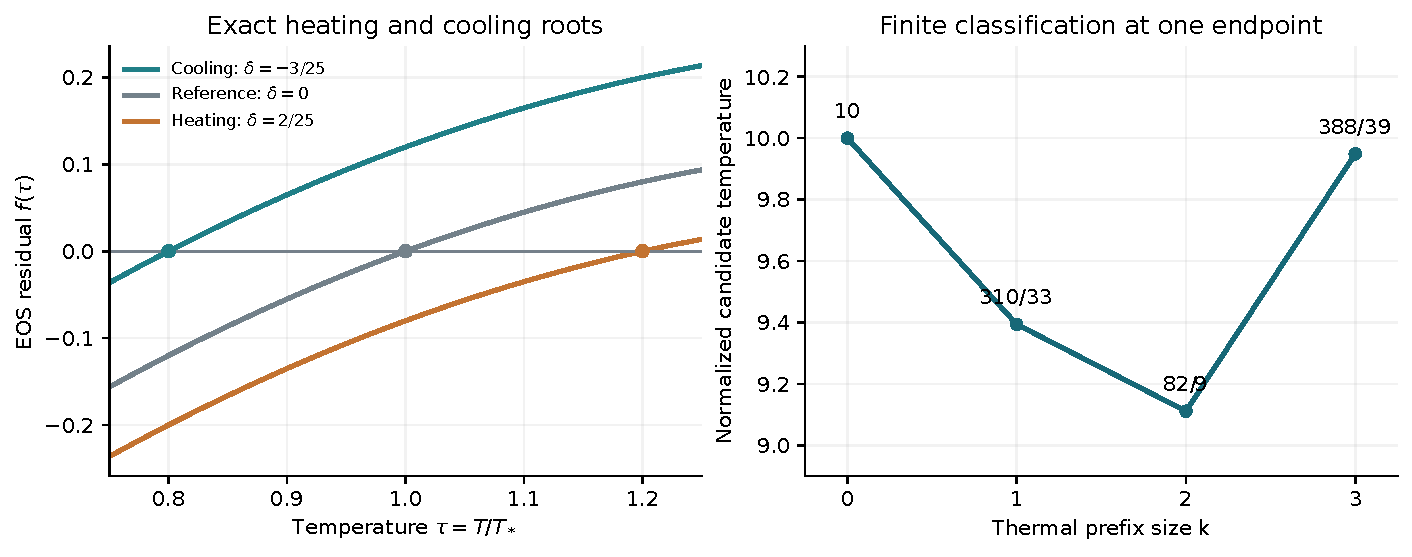
\includegraphics[width=\linewidth]{../figures/cutoff_construction.pdf}
\caption{연속 cutoff의 정확한 EOS 근과 원자 branch의 유한 편입. 오른쪽 가로축은 한 endpoint 안의 분류 후보 순서이며 물리 시간 단계가 아니다.}
\end{figure}

\hypertarget{uxc2e4uxc81c-uxaca9uxc790uxc758-uxc6d0uxc790-branch}{%
\subsection{실제 격자의 원자 branch}\label{uxc2e4uxc81c-uxaca9uxc790uxc758-uxc6d0uxc790-branch}}

\(\mu=\sum_jn_j\delta_{w_j}\)에는 미분 가능한 cutoff density를 가정하지 않고 prefix를 직접 사용한다. 첫 \(k\)개 node를 thermal로 둔 candidate는

\[
T_k=\frac{U_B+\sum_{j\le k}w_jn_j}{c_v(N_B+\sum_{j\le k}n_j)}
\]

이며 \(w_k\le\chi k_BT_k<w_{k+1}\)를 만족하면 consistent하다. \(M+1\)개 prefix를 검사하면 모든 해를 얻는다. \(\chi\ge3/2\)에서는 가장 낮은 에너지부터 조건에 맞는 원자를 편입하는 scan이 최대 \(M\)번에 끝남을 증명했다.

기존 branch에서 base energy만 변화시키면 가열은 위쪽 node의 편입, 냉각은 가장 높은 thermal node의 회수로 이어 간다. 양의 base를 유지하는 이 경로는 \(h=0\)에서 identity다. 새 원자를 편입한 직후 온도가 내려가더라도 그 원자가 여전히 cutoff 아래에 있다는 부등식이 유지되므로 scan은 성립한다.

Constructed example에서 \(N_B=10,U_B=15\), 원자 에너지 \((5,9,30)\), 각 count 1, \(\chi=4\)를 사용했다. Base energy에 135를 더하면 \(k:0\to1\to2\to3\)으로 끝나고, 다시 135를 빼면 \(3\to2\to1\to0\)으로 복귀한다. 일반적인 원자 spectrum에는 여러 branch가 존재할 수 있으므로 inherited branch와 모든 algebraic roots를 별도 출력한다.

\hypertarget{uxacf5uxbcc0-uxacbduxacc4uxc640-uxc804uxccb4-feedback}{%
\section{공변 경계와 전체 feedback}\label{uxacf5uxbcc0-uxacbduxacc4uxc640-uxc804uxccb4-feedback}}

Spectral number current가 \(\nabla_aj^a+\partial_W\mathcal F=\mathcal C\)를 만족하면, 움직이는 cutoff가 만드는 수 source는

\[
\boxed{S_c=j_c^a\nabla_aE_c-\mathcal F_c.}
\]

낮은 에너지 영역에는 \(S_c,E_cS_c\), 높은 영역에는 그 반대 부호가 들어간다. 경계 4-momentum의 시간 투영에서 rest mass를 빼면 운동에너지 전달 \(E_cS_c\)를 얻는다. \(j_c^a=c\rho_cn^a\)인 균질 경우에는 \(S_c=\chi k_B\rho_c\dot T-B_c\)로 기존 Bianchi 식과 연결된다.

Actual event extents \(\xi_r(z)\)로 raw inventory를 만든 뒤 cutoff EOS를 풀 때, 고정 cutoff의 thermal count·energy 증분을 \(\nu_{N,r},\nu_{U,r}\)로 쓰면

\[
\boxed{D_z\mathcal T=
\frac{\sum_r(\nu_{U,r}-c_v\mathcal T\nu_{N,r})D_z\xi_r}{C_{\rm eff}}.}
\]

이 식은 에너지 입력과 추가 열적 입자수의 효과를 함께 반영한다. \(C_{\rm eff}\)가 작아지면 같은 사건 오차에 대한 온도 응답과 density feedback이 커진다. CP.8--12는 이 식을 기존 사건량 Lipschitz bound와 합쳐 계산 가능한 수축상수 \(q\)로 만든다. \(q<1\)인 self-map에서는 inner EOS residual과 outer descriptor residual을 합친 오차를 \(1/(1-q)\)로 제어한다.

원자 표현에서는 prefix가 고정된 branch에 이 미분식과 수축 정리를 적용한다. Threshold crossing에는 유한 branch algorithm을 사용한다. 연속 표현을 쓰면 trial과 독립인 고정 선형 기저 또는 그보다 일반적인 표현의 추가 응답을 명시해야 한다.

\hypertarget{uxc2e4uxc81c-uxac80uxc99d-uxb3c5uxb9bd-uxac80uxd1a0uxc640-uxd574uxc11d-uxbc94uxc704}{%
\section{실제 검증, 독립 검토와 해석 범위}\label{uxc2e4uxc81c-uxac80uxc99d-uxb3c5uxb9bd-uxac80uxd1a0uxc640-uxd574uxc11d-uxbc94uxc704}}

\hypertarget{uxc774uxbc88uxc5d0-uxc2e4uxd589uxd55c-uxac80uxc0b0}{%
\subsection{이번에 실행한 검산}\label{uxc774uxbc88uxc5d0-uxc2e4uxd589uxd55c-uxac80uxc0b0}}

\begin{longtable}[]{@{}
  >{\raggedright\arraybackslash}p{(\columnwidth - 4\tabcolsep) * \real{0.3333}}
  >{\raggedright\arraybackslash}p{(\columnwidth - 4\tabcolsep) * \real{0.3333}}
  >{\raggedright\arraybackslash}p{(\columnwidth - 4\tabcolsep) * \real{0.3333}}@{}}
\toprule\noalign{}
\begin{minipage}[b]{\linewidth}\raggedright
검산 대상
\end{minipage} & \begin{minipage}[b]{\linewidth}\raggedright
실제 결과
\end{minipage} & \begin{minipage}[b]{\linewidth}\raggedright
근거
\end{minipage} \\
\midrule\noalign{}
\endhead
\bottomrule\noalign{}
\endlastfoot
9600-grid 및 source identity & 실제 energy array digest 일치; 11개 원본 파일 결속 & \texttt{KERNEL\_SOURCE\_BINDING} \\
실제 사건 열 & 17개 열 × 4개 invariant residual 모두 exact zero & \texttt{KERNEL\_ADAPTER\_CHECKS} \\
원래 floating projector와 exact layer & 최대 scale-normalized 차이 \(8.42\times10^{-14}\) & 같은 기록 \\
같은 family sharing 유지 & 실제 세 sharing points의 \(\xi_\ell/p_\ell\) exact equality & \texttt{SHARING\_CAPACITY\_CHECKS} \\
연속 cutoff reference & 가열 37회, 냉각 39회 이분; 각각 오차 \(7.28\times10^{-13}\), \(1.82\times10^{-13}\) in \(T/T_*\) & \texttt{THERMAL\_CUTOFF\_CHECKS} \\
원자 branch reference & 가열·냉각, equality, 복수 branch, \(h=0\) 통과 & 같은 기록 \\
Wolfram scalar & 17개 zero group, 21개 scalar residual=0; 부등식 5개 참 & \texttt{WOLFRAM\_SCALAR\_RAW} \\
Wolfram 안의 xAct & 새 tensor residual 6개 모두 0 & \texttt{WOLFRAM\_XACT\_RAW} \\
\end{longtable}

Wolfram kernel은 15.0.1, xTensor는 1.3.0, xPerm은 1.2.4였다. 공식 package bytes의 SHA256을 확인하고 pure Wolfram Language permutation 경로를 사용했다. xAct는 실제로 정의한 4차원 계량, 공변미분, 단위 시간벡터와 수 전류를 대상으로 selector product, partition cancellation, stress product, rest-mass energy subtraction, temperature cutoff current를 계산했다. 약한 분포 극한과 고정점 정리의 증명은 본문의 수학적 전제와 논증에 있다.

계산 도중 WolframContext의 내부 서비스 오류 1건이 있었으며 evaluator와 xAct 실행은 이어서 성공했다. 첫 scalar harness에서 \texttt{ForAll} 내부의 inline derivative 평가가 두 부등식에 잘못된 결과를 내어, 미분을 먼저 계산한 표현과 literal derivative를 대조했다. 그 진단에 따라 해당 두 구문을 고치고 새 canonical batch를 한 번 재실행했다. 최초 출력, 진단, 최종 출력을 모두 보존했다.

Actual-kernel의 큰-step 사례는 정확한 유한 장부와 양수성의 stress witness다. 여기서 나온 100 K→103.815911 K는 해당 구성 상태의 EOS 값이다. 그 step의 물리 시간 정확도나 새로운 우주론적 온도 예측을 뜻하지 않는다. 이전 unit의 과학 suite는 재실행하지 않았고, 전체 generator·새 물리 ODE·NCP job도 이번에 실행하지 않았다.

\hypertarget{uxb3c5uxb9bd-uxac80uxd1a0uxac00-uxbcf4uxc644uxd55c-uxc804uxc81c}{%
\subsection{독립 검토가 보완한 전제}\label{uxb3c5uxb9bd-uxac80uxd1a0uxac00-uxbcf4uxc644uxd55c-uxc804uxc81c}}

KC1--KC7은 명시된 가정 범위에서 모두 \texttt{PROMOTE\_SCOPED\ /\ PASS}를 받았다. 심사에서 지적한 9개 항목은 모두 닫혔으며, 72개 근거 파일의 정확한 bytes를 동결했다. 최상위 주장·전제 기록의 판정 metadata 갱신은 과학 본문 hash와 별도로 결속했다.

독립 검토자는 유도·원본 함수·실행 code·actual raw output을 직접 대조했다. 높은 에너지 영역의 부분적분에는 \(W\mathcal F(W)\to0\) 조건을 추가했고, CP의 연속 event reconstruction은 trial과 독립인 고정 선형 기저라는 전제를 명시했다. 문서의 비음성 표현과 \(U\ge0\Rightarrow T\ge0\)를 정밀화했다. Lipschitz 계수에 대한 CP bound는 고정 trial temperature의 root perturbation으로 직접 증명했다. 각 교정은 해당 범위를 유지하는 최소 보완이다.

\hypertarget{uxbb3cuxb9ac-uxc801uxc6a9uxc5d0-uxc804uxb2ecuxd560-uxc870uxac74}{%
\subsection{물리 적용에 전달할 조건}\label{uxbb3cuxb9ac-uxc801uxc6a9uxc5d0-uxc804uxb2ecuxd560-uxc870uxac74}}

Source는 HI·HeI cold-target full BED와 adopted excitation closure를 제공한다. HeII의 추가 이온화·재결합, finite-temperature diffusion, 모든 27개 여기 table에 대한 새 전체 generation은 각각 필요한 모형에서 추가하는 별도 입력이다. \(\chi\ge3/2\)는 원자 cutoff 해의 구성 조건이고, cold-target 정확도를 정량적으로 보장하는 조건은 아니다.

Source의 0.1 eV absorber 아래로 cutoff를 내려야 한다면 그 band의 실제 energy trace를 유지하거나 양의 reconstruction을 별도 결속해야 한다. Thermal 총 count·energy 두 값만으로 임의의 lower trace를 복원할 수는 없다. 이번 구현은 retained 원자 inventory를 명시적으로 유지하는 경로를 제공한다.

실제 적용에서 필요한 입력은 선택 source/history, \(\chi\)와 cutoff domain, thermal ownership, rate domain 및 이름·단위가 정해진 관측량 오차 예산이다. 현재 일반 이론의 성립 여부와 그 선택 응용의 물리 정확도는 각자의 근거로 판정한다.

\hypertarget{uxb2e4uxc74c-uxc5f0uxad6cuxacc4uxd68d}{%
\section{다음 연구계획}\label{uxb2e4uxc74c-uxc5f0uxad6cuxacc4uxd68d}}

기존 DAG의 \nolinkurl{CR_THEORY_KERNEL_EVENT_ADAPTER}와 \nolinkurl{CR_THEORY_THERMAL_CUTOFF_FEEDBACK}를 이번 결과에 연결했다. 다음 순서는 다음과 같다.

\begin{longtable}[]{@{}
  >{\raggedright\arraybackslash}p{(\columnwidth - 4\tabcolsep) * \real{0.3333}}
  >{\raggedright\arraybackslash}p{(\columnwidth - 4\tabcolsep) * \real{0.3333}}
  >{\raggedright\arraybackslash}p{(\columnwidth - 4\tabcolsep) * \real{0.3333}}@{}}
\toprule\noalign{}
\begin{minipage}[b]{\linewidth}\raggedright
다음 노드
\end{minipage} & \begin{minipage}[b]{\linewidth}\raggedright
바로 수행할 첫 구성
\end{minipage} & \begin{minipage}[b]{\linewidth}\raggedright
완료 기준
\end{minipage} \\
\midrule\noalign{}
\endhead
\bottomrule\noalign{}
\endlastfoot
Coupled branch solver & 실제 HI·HeI subfamily, retained atoms, CP.3 모멘트로 한 branch의 온도·전자밀도·조성 endpoint를 함께 구성 & 실제 domain과 self-map, 잔차 예산, 한 threshold crossing의 보존·branch 선택 \\
Geometry 이후 kernel 재결속 & prescribed Bianchi redshift로 바뀐 actual parent energy에 daughter projector와 rate domain을 다시 결속 & geometry work와 cutoff source의 단일 장부, 현재 energy identity 및 representation error \\
선택 응용 & 실제 source/history와 관측량의 허용오차를 앞의 결과에 연결 & 해당 source와 receiver 범위의 물리·수치 오차 근거 \\
\end{longtable}

이론의 다음 두 구성은 일반 입력으로 시작할 수 있다. 선택 응용은 기존 DAG에 남아 있는 source/scenario 및 observable budget의 의존성을 사용한다. 다음 세션에서는 \texttt{HANDOFF.json}과 \texttt{NEXT\_DAG.json}을 읽고 현재 동결 근거를 재사용한다.

\hypertarget{uxc5f0uxad6c-uxb8e8uxd504-uxc218uxd589-uxae30uxb85d}{%
\subsection{연구 루프 수행 기록}\label{uxc5f0uxad6c-uxb8e8uxd504-uxc218uxd589-uxae30uxb85d}}

R1 계약과 두 열린 노드 선택, R2 원본·이전 근거 재사용, R3 주장·전제 분리, R4 연속·원자 표현의 비교, R5 실제 구성과 증명, R6 독립 검토, R7 판별 계산, R8 범위별 판정, R9 reference 구현·정식 보고서, R10 DAG·source·인계본을 연결했다. C1--C10은 같은 식·입력에서 유도된 작은 구현, exact reference, source identity 및 독립 코드 검토로 이어진다. 단계별 근거 위치는 \texttt{policy/LOOP\_RECORD.json}에 있다.

\hypertarget{uxc804uxccb4-uxc720uxb3c4}{%
\section{전체 유도}\label{uxc804uxccb4-uxc720uxb3c4}}

다음 세 장은 실제 원자 source에서 시작하는 KA, 온도 의존 finite cutoff의 TCF, 공변 경계와 전체 결합 bound의 CV·CP를 수록한다. 첫머리의 결과 설명과 같은 수식·범위를 사용한다.

\clearpage

\hypertarget{uxc2e4uxc81c-bass_cr-daughter-kerneluxc5d0uxc11c-uxbcf4uxc874-uxc0acuxac74-uxc5f4uxb85c-uxac00uxb294-uxad6cuxc131}{%
\section{실제 BASS\_CR daughter kernel에서 보존 사건 열로 가는 구성}\label{uxc2e4uxc81c-bass_cr-daughter-kerneluxc5d0uxc11c-uxbcf4uxc874-uxc0acuxac74-uxc5f4uxb85c-uxac00uxb294-uxad6cuxc131}}

연구 단위: \nolinkurl{CR-THEORY-KERNEL-CUTOFF-20261013}\\
노드: \nolinkurl{CR_THEORY_KERNEL_EVENT_ADAPTER}\\
기준 commit: \nolinkurl{1f32987b2cc3eb521b4e09c736873ce21e9657a4}\\
의존 근거: 승인된 FB1--FB7의 shared-capacity map, endpoint feedback 정리, covariant geometry 구성. 이 문서는 이들을 실제 PHYS02C/PHYS02B kernel에 결속하는 새 유도이다.

\hypertarget{uxc774uxbc88uxc5d0-uxb2ebuxb294-uxb300uxc0c1uxacfc-uxc2e4uxc81c-uxc785uxb825}{%
\subsection{이번에 닫는 대상과 실제 입력}\label{uxc774uxbc88uxc5d0-uxb2ebuxb294-uxb300uxc0c1uxacfc-uxc2e4uxc81c-uxc785uxb825}}

선택한 물리 모형은 PHYS02B의 전자 stopping·projection·CCC excitation에 PHYS02C의 coherent full BED HI/HeI ionization을 결합한 기존 모형이다. 실제 저장된 9600-node array와 실제 source definitions를 읽었다. 원래의 외부 proton/electron injection이나 전체 time evolution을 재실행하지 않고, collision operator의 사건 분해 및 조성 feedback을 구성한다.

\begin{longtable}[]{@{}
  >{\raggedright\arraybackslash}p{(\columnwidth - 4\tabcolsep) * \real{0.3333}}
  >{\raggedright\arraybackslash}p{(\columnwidth - 4\tabcolsep) * \real{0.3333}}
  >{\raggedright\arraybackslash}p{(\columnwidth - 4\tabcolsep) * \real{0.3333}}@{}}
\toprule\noalign{}
\begin{minipage}[b]{\linewidth}\raggedright
근거 ID
\end{minipage} & \begin{minipage}[b]{\linewidth}\raggedright
실제 Git 경로
\end{minipage} & \begin{minipage}[b]{\linewidth}\raggedright
이번 역할
\end{minipage} \\
\midrule\noalign{}
\endhead
\bottomrule\noalign{}
\endlastfoot
SRC-P & \nolinkurl{research/cr_phys02b_20261010/src/causal_cascade.py} & \texttt{Cascade.project}, \texttt{\_sharing}, \texttt{stopping\_eV\_s}, generator의 열 조립식 \\
SRC-B & \nolinkurl{research/cr_phys02c_20261011/src/coherent_bed.py} & HI/HeI coherent full BED total/SDCS \\
SRC-G & \nolinkurl{research/cr_phys02c_paired_9600_closeout_20261011/raw/THIRD_GRID_LOCAL_20261011_EXEC01/SPECTRUM_fullBED_9600.npz} & 실제 저장된 \texttt{energy\_eV} \\
SRC-C & \nolinkurl{research/cr_phys02b_20261010/inputs/CCC_USED_CHANNELS.json} & 27개 기존 channel·단위·effective cost inventory \\
SRC-H & \nolinkurl{research/cr_phys02b_20261010/inputs/ccc/HI/2P.1S} & 실제 HI 1S→2P table \\
SRC-He & \nolinkurl{research/cr_phys02b_20261010/inputs/ccc/HeI/t2S.s1S} & 실제 HeI s1S→t2S table \\
SRC-O & \nolinkurl{research/cr_phys02c_20261011/research/ionization_sources/SOURCE_ALGEBRA_RESULT.json} & 기존 oscillator algebra의 채택 상수 \\
\end{longtable}

전체 11개 결속 파일의 Git blob SHA-1, SHA-256, bytes는 \nolinkurl{inputs/KERNEL_SOURCE_BINDING.json}에 있다. 복원된 local source bytes를 현재 pinned tree의 blob identity와 각각 대조했다. NPZ SHA-256은 \nolinkurl{7ee8c1eff7f58cd7175a9bcd3968a27ef065f0e983f05e609dc875f5f06112cc}이고, 저장된 \texttt{\textless{}f8}, C-order \texttt{energy\_eV} 9600개의 raw SHA-256은 \nolinkurl{6a76d3539115003b046a5861baca89b0a4ff966564627e04d9f6e8bc86be8292}이다. 첫 node는 0.10309375000000001 eV, index 3199는 10 eV, 마지막은 900 eV다. 새 mesh를 생성하거나 저장된 spectrum을 다시 구하지 않았다.

고정한 source 상수는

\[
 W_b=0.1\ {\rm eV},\quad W_{\max}=900\ {\rm eV},\quad
 B_H=13.6057\ {\rm eV},\quad B_{He}=24.587\ {\rm eV},
 \tag{KA.1}
\]

이며 atomic 대상은 HI와 HeI이다. HeII의 추가 ionization rate, recombination rate, thermal-ionization rate는 이 source가 제공하는 이번 event family에 포함되지 않는다. 기존 FB family는 그런 사건을 더할 수 있는 구조 정리로 재사용하고, 실제 원자 자료의 범위는 위 두 종에 결속한다.

원래 고정 bath의 수밀도는 \(n_{HI,0}=138.6\ {\rm m}^{-3}\), \(n_{HeI,0}=11.427127659574467\ {\rm m}^{-3}\), \(n_{e,0}=1.5154255319148937\ {\rm m}^{-3}\), 원래 gas temperature는 100 K이다. 새 continuation에서는 target neutral counts와 thermal electron count를 갱신한다. 이때 stopping에 들어가는 \(n_e\)는 \textbf{thermal electron bath의 수밀도}로 명시한다. 핵종을 포함한 EOS의 전체 thermal particle count 또는 active electron까지 포함한 전체 자유전자 수밀도와 구별한다.

\hypertarget{uxc0c1uxd0dcuxc640-lower-absorberuxc758-uxd45cuxd604}{%
\subsection{상태와 lower absorber의 표현}\label{uxc0c1uxd0dcuxc640-lower-absorberuxc758-uxd45cuxd604}}

고정 physical volume \(V_*>0\)에서 저장된 grid node를 \(W_j\), 그 node의 raw count를 \(A_j\)라 하자. source eV를 SI energy로 바꾸는 상수는 \(\epsilon_{\rm eV}=1.602176634\times10^{-19}\ {\rm J/eV}\)이며, \(\mathcal W_j=\epsilon_{\rm eV}W_j\)로 쓴다. 표기상의 eV 좌표와 별도로 상태의 energy 좌표는 SI J로 유지한다.

Raw node measure와 source lower absorber를 분리한 상태는

\[
 y=(\{A_j\},X_H,X_{H^+},X_{He},X_{He^+},N_{e,B},U_B,
                   E_{exc,H},E_{exc,He})\ge0.
 \tag{KA.2}
\]

여기서 \(N_{e,B},U_B\)는 source의 \(W\le W_b\) absorber와 이미 분해되지 않는 thermal bath에 남긴 count/energy이다. \(U_B\)에는 해당 bath의 열적 에너지가 들어간다. Source의 \texttt{heat}와 \texttt{cutoff\_energy}는 각각 감사 가능한 관측 장부로 보존하면서, 물리 상태에는 그 합을 \(U_B\)에 한 번만 더한다. 이미 ion stage count의 chemical energy로 계산한 \texttt{binding} 역시 에너지 합에 중복해서 더하지 않는다.

물리적 active cutoff \(E_c^n\)가 \(\epsilon_{\rm eV}W_b\) 이상인 결합에서는 raw \(A_j\)에 thermal-owned retained atoms도 들어갈 수 있다. Collision의 초기 donor mask는

\[
 m_j^n=\mathbf1_{\{\mathcal W_j>E_c^n\}},\qquad
 A_{j,\mathrm{donor}}^n=m_j^n A_j^n.
 \tag{KA.3}
\]

으로 고정한다. Trial endpoint cutoff가 변해도 이 초기 mask나 사건 열을 누적 수정하지 않는다. 매 trial은 같은 collision raw output을 분류한다. 선택된 thermal-owned atoms를 \(\mathcal I_{th}\)라 할 때

\[
 N_{e,th}=N_{e,B}+\sum_{j\in\mathcal I_{th}}A_j,\qquad
 U_{th}=U_B+\sum_{j\in\mathcal I_{th}}\mathcal W_jA_j,
 \tag{KA.4}
\]

이며 \(N_{th}=X_H+X_{H^+}+X_{He}+X_{He^+}+N_{e,th}\)를 EOS에 사용한다. Raw inventory를 유지하는 표현과 aggregate \(U_{th},N_{e,th}\) 표현 사이를 변환할 때 (KA.4)의 atom 기여를 두 번 세지 않는다. 이번 source absorber는 \(W_b\) 아래의 \textbf{각 actual energy trace}를 저장하지 않으므로, 그 band를 다시 통과하는 하향 cutoff에는 trace를 추가 보존하거나 cutoff domain을 제한해야 한다. 원래 source semantics를 보존한 이번 adapter는 그 조건을 인터페이스에 남긴다.

\hypertarget{uxae30uxc874-projectoruxc758-uxc591uxc758-countenergy-uxbd84uxd574}{%
\subsection{기존 projector의 양의 count--energy 분해}\label{uxae30uxc874-projectoruxc758-uxc591uxc758-countenergy-uxbd84uxd574}}

한 daughter energy \(w\)에 대해 count projector \(P_N(w)=(\{b_i(w)\},n_B(w),u_B(w))\)를 정의한다. 이는 SRC-P의 energy-coordinate projector를 count coordinate로 읽은 것이다.

\(0\le w\le W_b\)이면

\[
 b_i(w)=0,\quad n_B(w)=1,\quad u_B(w)=w.
 \tag{KA.5a}
\]

\(W_b<w\le W_{\max}\)이면 \(w\)를 감싸는 두 source nodes \(\ell\le w\le u\)를 잡고

\[
 \beta={w-\ell\over u-\ell},\qquad
 P_N(w)=(1-\beta)P_N(\ell)+\beta P_N(u),\quad0\le\beta\le1.
 \tag{KA.5b}
\]

내부 grid node는 그 node에 한 count를 넣는다. 첫 active node 아래에서는 \(\ell=W_b\)를 ghost absorber로 읽어, \((1-\beta)\) count와 \((1-\beta)W_b\) energy를 base에 넣는다. 따라서 source는 \(W_b<w<W_0\)에서도 작은 ghost fraction을 쓴다. 이는 원래의 first-cell closure다. 이 ghost contribution은 실제 \(w\le W_b\) daughter가 전부 흡수된 경우와 출력 JSON에서 별도로 기록한다.

각 분해의 계수는 비음수이고,

\[
 \sum_i b_i(w)+n_B(w)=1,\qquad
 \sum_iW_i b_i(w)+u_B(w)=w.
 \tag{KA.6}
\]

증명은 내부 cell에서 \((1-\beta)+\beta=1\), \((1-\beta)\ell+\beta u=w\)이고, lower absorber에서는 (KA.5a)를 대입하면 끝난다. 임의의 양의 daughter weights에 선형으로 확장된다. Grid spacing이 \(\Delta_{\min}>0\)이면 한 cell에서 count 계수의 \(\ell^1\) 변화율은 \(2/\Delta\le2/\Delta_{\min}\)이다. 이 bound는 exact rational completion과 원래 float evaluation 사이의 작은 energy-rounding 차이를 비교하는 데에도 쓰인다.

\hypertarget{uxc2e4uxc81c-full-beduxc5d0uxc11c-uxc591uxc758-quadrature-weights}{%
\subsection{실제 full BED에서 양의 quadrature weights}\label{uxc2e4uxc81c-full-beduxc5d0uxc11c-uxc591uxc758-quadrature-weights}}

SRC-B의 \(t=E/B>1\), \(w=W/B\), \(u=U/B\), \(y=(1+w)^{-1}\), \(r=(t-w)^{-1}\)에 대해 SDCS는

\[
 {d\sigma\over dW}={S\over B(t+u+1)}
 \left\{K\left[y^2+r^2-{y+r\over t+1}\right]
                  +{\log t\over N}g(w)y\right\}.
 \tag{KA.7}
\]

원래 상수에서 \(K=2-N_i/N>0\)이다. 또 \(y+r=(t+1)yr\)이므로 첫 항의 대괄호는

\[
 y^2+r^2-yr=(y-r)^2+yr>0.
 \tag{KA.8}
\]

HI oscillator는 source의 양의 exponential/rational 식이며 \(w=0\)의 연속 값도 \(128/(3e^4)>0\)이다. HeI에서는

\[
 g(w)=y^3 q(y),\quad q(y)=8.24012-10.4769y+3.96496y^2-0.0445976y^3.
 \tag{KA.9}
\]

\(0<y\le1\)에서 \(q'(y)=-10.4769+7.92992y-0.1337928y^2<0\), \(q(1)=1.6835824>0\)이므로 \(g>0\)이다. 따라서 허용된 slow-electron interval 전체에서 (KA.7)은 양수다.

Total cross section의 source식도

\[
 \sigma(E)={S\over t+u+1}\left[D(t)\log t+
     K\left(1-{1\over t}-{\log t\over t+1}\right)\right]\ge0
 \tag{KA.10}
\]

이다. \(D(t)\)는 \(g(w)/(N(1+w))\)의 양의 적분이다. 나머지 함수 \(H(t)=1-t^{-1}-\log t/(t+1)\)는 \(H(1)=0\),

\[
 H'(t)={t+1+t^2\log t\over t^2(t+1)^2}>0\quad(t>1)
\]

을 만족한다. Threshold 이하에는 source가 rate를 0으로 둔다. 원래 source의 oscillator integral 및 total/SDCS 일치는 채택한 SRC-O 근거를 재사용한다.

Source \texttt{\_sharing}은 \([0,(E_j-B_a)/2]\)에 기존 grid knots와 reflected knots를 함께 넣고, 각 interval에 order-4 Gauss--Legendre rule을 적용한다. 실제 sampling energies를 \(w_{ja\ell}\), 양의 raw quadrature weight를 \(q_{ja\ell}\)라 하면

\[
 p_{ja\ell}={q_{ja\ell}\over\sum_\nu q_{ja\nu}}>0,\qquad
 \sum_\ell p_{ja\ell}=1.
 \tag{KA.11}
\]

이번 구현은 그 함수를 변경 없이 읽어 사용한다. 이 식은 원래 total rate \(\sigma_a(E_j)\)를 각 공유 사건에 분배하며, 새로운 cross section을 가정하지 않는다.

\hypertarget{paired-fractional-ionization-event}{%
\subsection{Paired fractional ionization event}\label{paired-fractional-ionization-event}}

Species \(a\in\{H,He\}\), parent \(j\), 실제 sharing point \(\ell\)에 대해

\[
 w_1=w_{ja\ell},\qquad w_2=E_j-B_a-w_1
\]

를 같은 사건 안에 둔다. 두 projector를 합쳐 \(b_i=b_i(w_1)+b_i(w_2)\), \(n_B=n_B(w_1)+n_B(w_2)\), \(u_B=u_B(w_1)+u_B(w_2)\)라 쓰면 그 사건 열은

\[
 \Delta A_i=-\delta_{ij}+b_i,\quad
 \Delta X_a=-1,\quad\Delta X_{a^+}=1,\quad
 \Delta N_{e,B}=n_B,\quad\Delta U_B=\epsilon_{\rm eV}u_B.
 \tag{KA.12}
\]

\(X_a^n>0\)인 초기 support에서 실제 trial composition proposal은

\[
 f_{ja\ell}(z;y^n)=m_j^n A_j^n\,
       v_j\sigma_a(E_j)p_{ja\ell}{X_a(z)\over V_*},\qquad
 v_j=\sqrt{2\epsilon_{\rm eV}E_j/m_e}.
 \tag{KA.13}
\]

이 식의 속도는 SRC-P의 비상대론적 prescription을 그대로 쓴다. \(X_a^n=0\) 또는 \(m_j^nA_j^n=0\)인 채널은 그 step에서 비활성이다. 기존 frozen-mass factor \(A_j^nX_a^n/V_*\)를 유지하려면 \(\widehat\kappa(z)=v_j\sigma_a p_{ja\ell}X_a(z)/X_a^n\)로 읽으면 같은 식이다. Trial target를 \(X_a^n\)에 고정한 것은 이 구성의 더 단순한 특수 경우다. \(z=y^n\)에서는 정확히 \(A_j^n n_a^n v_j\sigma_a p_{ja\ell}\)이므로 원래 continuous mass-action rate와 일치한다.

(KA.6)에서 곧바로

\[
 \sum_i\Delta A_i+\Delta N_{e,B}=1,
\quad
 \sum_i\epsilon_{\rm eV}W_i\Delta A_i+\Delta U_B+\epsilon_{\rm eV}B_a\Delta X_{a^+}=0
 \tag{KA.14}
\]

가 따른다. 핵종 수는 \(\Delta X_a+\Delta X_{a^+}=0\)이고, ion charge가 1 늘면서 자유전자도 1 늘므로 전하가 보존된다. 두 daughter를 합친 열의 계수는 fractional counts일 수 있다. 이것은 mean-measure deterministic event이며, 정수-valued Monte Carlo collision을 주장하는 것이 아니다. 두 daughter를 따로 독립적인 grid outcome으로 추첨하는 분해를 사용하지 않으므로 각 사건 열이 에너지 관계를 유지한다.

\hypertarget{uxc2e4uxc81c-ccc-excitationuxacfc-stopping-uxc0acuxac74}{%
\subsection{실제 CCC excitation과 stopping 사건}\label{uxc2e4uxc81c-ccc-excitationuxacfc-stopping-uxc0acuxac74}}

SRC-C의 excitation 채널 \(c\)는 native zero marker를 effective energy loss \(C_c>0\)로 쓴다. Native sigma를 HI의 \(a_0^2\)이면 \(a_0^2\), HeI의 \({\rm cm}^2\)이면 \(10^{-4}\)를 곱해 \({\rm m}^2\)로 변환하고 piecewise-linear interpolation을 적용한다. 표본 sigma가 비음수이므로 interpolated sigma도 비음수이다. Lower marker 아래는 0이고, 선정 domain은 마지막 tabulated energy 이하다.

Excitation의 한 사건은

\[
 \Delta A_i=-\delta_{ij}+b_i(E_j-C_c),\quad
 \Delta N_{e,B}=n_B(E_j-C_c),\quad
 \Delta U_B=\epsilon_{\rm eV}u_B(E_j-C_c),\quad
 \Delta E_{exc,a}=\epsilon_{\rm eV}C_c.
 \tag{KA.15}
\]

핵종·ion stage count는 그대로이며 proposal은 (KA.13)에서 \(\sigma_ap_{ja\ell}\)를 \(\sigma_c\)로 바꾼다. Neutral target는 rate의 co-reactant이고, 이 effective excitation/radiation closure에서 그 neutral count의 \textbf{net increment}는 0이다. 따라서 capacity matrix에 가상의 neutral depletion을 추가하지 않는다. \(\Delta N_{free}=0\)이고 \(\Delta E_{kin}+\Delta U_B+\Delta E_{exc}=0\)이다. 이번에 직접 평가한 effective cost는 HI 1S→2P의 10.20435 eV와 HeI s1S→t2S의 19.7179 eV다. 이는 source가 채택한 truncated model cost라는 의미를 보존한다. 별도의 정확한 spectroscopic transition energy 또는 excited population kinetics로 확대 해석하지 않는다.

Stopping은 \(E_{j-1}\)를 이전 node, 첫 node에서는 \(E_{-1}=W_b\)로 두고

\[
 \Delta A_i=-\delta_{ij}+b_i(E_{j-1}),\quad
 \Delta N_{e,B}=n_B(E_{j-1}),\quad
 \Delta U_B=\epsilon_{\rm eV}\{u_B(E_{j-1})+E_j-E_{j-1}\},
 \tag{KA.16}
\]

\[
 f_j^{stop}(z;y^n)=m_j^nA_j^n\lambda_j(n_e(z)),\qquad
 \lambda_j(n_e)={b(E_j,n_e)\over E_j-E_{j-1}}.
 \tag{KA.17}
\]

로 정한다. 내부 node에서는 한 active electron이 이전 node로 가고 차이만 heat가 된다. 첫 node에서는 한 thermal electron을 추가하고 총 \(\epsilon_{\rm eV}E_0\)를 \(U_B\)에 넣는다. 그중 \(\epsilon_{\rm eV}W_b\)는 source cutoff-energy 장부, 나머지는 source heat 장부라는 분해가 그대로 남는다. Count와 에너지 보존은 (KA.6)을 대입하면 각각 0이다.

\hypertarget{uxc6d0uxb798-generatoruxc640uxc758-uxc77cuxce58}{%
\subsection{원래 generator와의 일치}\label{uxc6d0uxb798-generatoruxc640uxc758-uxc77cuxce58}}

원래 SRC-P는 active energy-density coordinate \(u_j=E_jA_j/V_*\)와 energy/number observers에 행렬 \(G\)를 작용시키며, 저장한 \(G\)에는 \(T_{END}\) factor가 들어간다. Physical generator는 \(G/T_{END}\)다. 고정 원래 bath로 (KA.13), (KA.17)을 평가하고 모든 sharing events를 더하면

\[
 {dA_i\over dt}=\sum_r S_{ir} f_r,\qquad
 {du_i\over dt}={E_i\over V_*}\sum_r S_{ir} f_r.
 \tag{KA.18}
\]

Parent energy-coordinate 한 단위에 해당하는 count는 \(V_*/E_j\)이므로 source column은 정확히 \(-\lambda_j\)와 \(\lambda_j P_E/E_j\) 형식을 얻는다. Ionization의 binding observer에는 \(\lambda_aB_a/E_j\), ionization-number observer에는 \(\lambda_a/E_j\), excitation observer에는 \(\lambda_cC_c/E_j\), stopping heat에는 \(\lambda_j(E_j-E_{j-1})/E_j\)가 들어간다. 이는 SRC-P \texttt{\_generator}의 실제 조립식 각각과 일치한다. 원래 \texttt{low\_cross\_energy/number}는 이미 센 성분의 겹치는 관측량이므로 독립 보존 energy에 더하지 않는다.

따라서 이 adapter는 선택된 원래 discrete collision generator를 count·species·thermal 상태의 공통 사건 표현으로 확장한다. 원래 고정 bath를 회복하면 그 active/observer operator가 돌아오고, trial composition을 켜면 같은 사건 열에 nonlinear rate가 연결된다.

\hypertarget{uxc2e4uxc81c-stopping-feedbackuxc640-rate-derivative-bound}{%
\subsection{실제 stopping feedback와 rate derivative bound}\label{uxc2e4uxc81c-stopping-feedbackuxc640-rate-derivative-bound}}

Source의 Coulomb 상수는 \(\mathcal K=e^2/(4\pi\epsilon_0)\)이며 \(e=1.602176634\times10^{-19}\ {\rm C}\)는 elementary charge이다. Energy-conversion 상수 \(\epsilon_{\rm eV}\)와 \(e\)의 SI 수치가 같지만 차원을 구별한다. Fixed \(E_j,v_j\)에 대해

\[
 \omega_p(n)=\sqrt{ne^2/(\epsilon_0m_e)},\quad
 L_j(n)=\min\left\{
 \log{v_jE_j\epsilon_{\rm eV}\over\mathcal K\omega_p(n)},
 \log{2E_j\epsilon_{\rm eV}\over\hbar\omega_p(n)}+q
 \right\},\quad q\in\{0,-\tfrac12\}.
 \tag{KA.19}
\]

실제 baseline의 \(q=0\)을 이번 witness에 사용한다. 두 log에 같은 \(-\frac12\log n\)이 들어가므로 fixed \(E_j\)에서 어느 branch가 작은지는 density에 의존하지 않는다. \(n_0=n_{e,0}\)로 두면

\[
 L_j(n)=L_j(n_0)-\tfrac12\log(n/n_0),\quad
 b_j(n)=\alpha_jnL_j(n),\quad
 \alpha_j={4\pi\mathcal K^2\over m_ev_j\epsilon_{\rm eV}}.
 \tag{KA.20}
\]

따라서

\[
 b'_j(n)=\alpha_j(L_j(n)-\tfrac12),\qquad
 b''_j(n)=-{\alpha_j\over2n}.
 \tag{KA.21}
\]

정의역 \(0<n_{min}\le n\le n_{max}\), \(L_j(n_{max})>0\)에서

\[
 M_j=\sup|\lambda'_j(n)|
 ={\alpha_j\over E_j-E_{j-1}}
 \max\{|L_j(n_{min})-\tfrac12|,|L_j(n_{max})-\tfrac12|\}
 \tag{KA.22}
\]

가 유한하다. Density continuation은

\[
 n_e(z)={N_{e,th}(z)\over V_*},\qquad
 L_{f_j^{stop}}\le m_j^n A_j^n M_j {L_{N_{e,th}}\over V_*}.
 \tag{KA.23}
\]

로 이전 FB Lipschitz contract에 들어간다. \(\|\delta z\|_{\infty,a}=\max_i|\delta z_i|/a_i\)에서 atomic proposal의 bound는

\[
 L_{f_{ja\ell}}={m_j^n A_j^n v_j\sigma_a(E_j)p_{ja\ell}\over V_*}a_{X_a},
 \quad
 L_{f_{jc}}={m_j^n A_j^n v_j\sigma_c(E_j)\over V_*}a_{X_a}.
 \tag{KA.24}
\]

이들은 target count에 선형이므로 이 bound는 직접적이다. 선택된 source에서는 fixed energy의 total/SDCS/CCC coefficient에 직접적인 \(T\) 의존이 없고, stopping도 thermal bath density 외에 \(T\)를 인자로 쓰지 않는다. 따라서 fixed \(E\), fixed target/electron density에서 \(\partial_T\kappa=0\)이다. Trial cutoff가 thermal ownership을 바꾸는 경우의 온도 간접 효과는 \(N_{e,th}(z)\)를 통해 (KA.23)에 들어간다. Atom branch가 고정된 곳은 이 count가 선형 함수이며, branch jump나 smooth spectral reconstruction에 관한 bound는 cutoff 분과의 contract를 사용한다.

원래 cold-target 모형의 유효범위는 active \(\mathcal W_j\gg k_BT\), positive Coulomb log, dilute targets, 선정된 0.1--900 eV domain 및 원래 excitation closure를 포함한다. \(W_b/(k_BT_0/\epsilon_{\rm eV})\simeq11.60\)이다. Cutoff 존재 정리의 \(\chi\ge3/2\) 조건은 cold-target 근사의 정량적 정확도 조건을 대신하지 않는다. Finite-temperature Coulomb diffusion, all-free-electron screening 또는 thermal cross-section average를 원하면 별도로 rate closure를 유도한다.

\hypertarget{uxae30uxc874-shared-capacity-mapuxc5d0-uxadf8uxb300uxb85c-uxc5f0uxacb0}{%
\subsection{기존 shared-capacity map에 그대로 연결}\label{uxae30uxc874-shared-capacity-mapuxc5d0-uxadf8uxb300uxb85c-uxc5f0uxacb0}}

각 사건 열을 모아 \(S\), \(C_{ir}=\max(-S_{ir},0)\), base stock \(y^n\)을 둔다. 초기 zero donor를 요구하는 채널은 끄고, 같은 trial \(z\)에서

\[
 c_i(z)=\sum_r C_{ir}f_r(z),\quad
 d_r(z)=\sum_{i:C_{ir}>0}{c_i(z)\over y_i^n},\quad
 \xi_r(z)={h f_r(z)\over1+h d_r(z)},\quad
 \mathcal F(z)=y^n+S\xi(z)
 \tag{KA.25}
\]

를 적용한다. 각 donor \(i\)에 대해 \(d_r\ge c_i/y_i^n\)인 같은 분모를 쓰므로

\[
 \sum_rC_{ir}\xi_r\le {h c_i\over1+h c_i/y_i^n},\qquad
 (\mathcal F(z))_i\ge{y_i^n\over1+h c_i/y_i^n}\ge0.
 \tag{KA.26}
\]

원래 ion target depletion, active parent depletion, thermal/chemical/observer increments는 한 \(\xi_r\)를 공유한다. 서로 다른 coordinate를 별도로 보정하지 않는다.

이번 family의 선형 invariant는

\[
 \begin{aligned}
 H_{tot}&=X_H+X_{H^+},\\
 He_{tot}&=X_{He}+X_{He^+},\\
 Q/e&=X_{H^+}+X_{He^+}-N_{e,B}-\sum_jA_j,\\
 E_{tot}&=\sum_j\mathcal W_jA_j+U_B+\epsilon_{\rm eV}B_HX_{H^+}
                     +\epsilon_{\rm eV}B_{He}X_{He^+}+E_{exc,H}+E_{exc,He}.
 \end{aligned}\tag{KA.27}
\]

앞 절의 사건별 등식으로 각 row \(\ell\)가 \(\ell^TS=0\)이므로, 모든 \(h\ge0\)와 trial \(z\)에서 \(\ell^T\mathcal F(z)=\ell^Ty^n\)이다. Thermal repartition도 (KA.4)로 동일 raw count·energy를 옮기므로 이 invariant를 유지한다. \(N_{th}>0\), \(U_{th}\ge0\)이면 \(T=2U_{th}/(3k_BN_{th})\)가 비음수 EOS를 준다. 온도 양수성 \(T>0\)에는 \(U_{th}>0\)가 필요하다. Stopping/ionization/source excitation events는 base thermal energy를 감소시키지 않는다.

Rate bound (KA.23)--(KA.24)를 FB의 \(L_c,L_d,L_\xi\) 식에 넣으면 그대로

\[
 L_{c_i}=\sum_r C_{ir}L_{f_r},\quad
 L_{d_r}=\sum_{i:C_{ir}>0}{L_{c_i}\over y_i^n},\quad
 L_{\xi_r}\le hL_{f_r}+h^2 F_rL_{d_r},\quad
 q_{FP}=\max_i{\sum_r|S_{ir}|L_{\xi_r}\over a_i}
 \tag{KA.28}
\]

를 얻는다. 지정된 invariant domain 안에서 \(q_{FP}<1\)이면 FB의 고정점 유일성·Picard 수렴·residual error bound가 적용된다. 각 proposal이 \(f(y^n;y^n)=R(y^n)\)이고 branch별로 locally Lipschitz이면 \(\xi=hf(y^n)+O(h^2)\), \(y^{n+1}=y^n+hSR(y^n)+O(h^2)\)이므로 사건 분해가 기존 first-order consistency를 보존한다. 강한 positivity는 큰 \(h\)에서도 성립하지만, 그 사실만으로 큰 시간 간격의 정확도를 주장하지 않는다.

\textbf{실제 sharing distribution의 보존.} 저장된 전체 grid의 최대 gap은 0.6325633326908928 eV로, 최소 ion binding 13.6057 eV보다 작다. 따라서 두 ion daughter 모두 \(w\le E_j-B_a<E_{j-1}\)이며, 그 projector의 active support는 parent node를 포함하지 않는다. 모든 \((j,a,\ell)\) 사건의 negative increments는 정확히 \(A_j\)와 \(X_a\)의 각 1이다. 그러므로 capacity denominator는 같은 \((j,a)\) 안에서 \(\ell\)에 의존하지 않아

\[
 \xi_{ja\ell}=p_{ja\ell}\,\Xi_{ja},\qquad
 \Xi_{ja}={h\,m_j^n A_j^n v_j\sigma_a(E_j)X_a(z)/V_*
  \over1+h\{c_{A_j}(z)/A_j^n+c_{X_a}(z)/X_a^n\}}.
 \tag{KA.29}
\]

가 성립한다. Active positive support에서 읽는 이 식은 큰 \(h\)에서도 각 ionization family의 실제 daughter sharing probability를 유지한다. Total family extent가 공통 capacity에 맞게 줄어든다. 다른 target species 및 다른 parent family 사이의 상대 extent에는 각각의 shared stock 조건이 반영된다. 최소 CCC effective cost 10.20435 eV도 최대 grid gap보다 크므로 excitation daughters 역시 parent node에 재투영되지 않는다.

\hypertarget{uxc2e4uxc81c-uxc0c8-uxacc4uxc0b0uxacfc-uxac80uxc99d-uxacb0uxacfc}{%
\subsection{실제 새 계산과 검증 결과}\label{uxc2e4uxc81c-uxc0c8-uxacc4uxc0b0uxacfc-uxac80uxc99d-uxacb0uxacfc}}

\texttt{kernel\_event\_adapter.py}는 11개 input hash를 확인하고 실제 saved array를 읽은 뒤, SRC-P/SRC-B에서 필요한 함수·class AST만 변경 없이 실행한다. Module-level 전체 atomic loading, source evaluation, \texttt{\_generator}, matrix exponential, ODE, NCP를 호출하지 않는다. 실제 선택한 node/채널에서 원래 sharing와 projector를 평가하고, 새 exact event construction을 비교했다.

\begin{longtable}[]{@{}
  >{\raggedright\arraybackslash}p{(\columnwidth - 4\tabcolsep) * \real{0.2727}}
  >{\raggedleft\arraybackslash}p{(\columnwidth - 4\tabcolsep) * \real{0.3636}}
  >{\raggedleft\arraybackslash}p{(\columnwidth - 4\tabcolsep) * \real{0.3636}}@{}}
\toprule\noalign{}
\begin{minipage}[b]{\linewidth}\raggedright
새 평가 대상
\end{minipage} & \begin{minipage}[b]{\linewidth}\raggedleft
실제 parent energy (eV)
\end{minipage} & \begin{minipage}[b]{\linewidth}\raggedleft
sharing points / 사건 역할
\end{minipage} \\
\midrule\noalign{}
\endhead
\bottomrule\noalign{}
\endlastfoot
HI threshold 바로 위 & 13.606407443000693 & 4 \\
HI 중간 node & 30.00976971818039 & 15620 \\
HeI threshold 바로 위 & 24.595094858493628 & 4 \\
HeI 중간 node & 30.00976971818039 & 6888 \\
HI 1S→2P & 10.205990538235602, 30.00976971818039 & 실제 table 두 점 \\
HeI s1S→t2S & 19.722795822410312, 30.00976971818039 & 실제 table 두 점 \\
stopping & 0.10309375000000001, 10, 30.00976971818039 & 세 실제 grid edge \\
\end{longtable}

위 네 ionization component에서 source-projected daughter count residual은 0이고, 에너지 상대 residual의 최대 절댓값은 \(1.19\times10^{-16}\)이다. 실제 sharing weights는 모두 양수다. 각 component의 first/last 및 source ghost band의 실제 quadrature sample을 고른 exact witnesses, CCC 사건 및 stopping을 합한 \textbf{17개 사건 열}에서 (KA.27)의 네 invariant residual은 Fraction arithmetic으로 모두 정확히 0이다.

Reference의 exact layer는 saved float inputs를 binary rational로 읽고, fast daughter를 \(E-B-w_1\)로 정확히 완성하며, barycentric weights 및 sharing probability의 합을 exact arithmetic으로 계산한다. 원래 floating projection과의 최대 scale-normalized 차이는 \(8.42\times10^{-14}\)이다. 이 차이는 고정된 grid interpolation의 rounding sensitivity와 일치하며, floating generator를 bitwise identical rational matrix라고 주장하지 않는다. Exact 사건 장부와 원래 floating implementation과의 수치 일치는 각각 별도 근거로 기록한다.

이 중 \textbf{7-event 실제 sparse subfamily}에 기존 \nolinkurl{inputs/prior/event_capacity_step.py}를 byte 그대로 사용했다. 초기 상태는 이번 검증용으로 구성한 neutral 상태이며 저장된 historical spectrum이 아니다. \(h=10^{14}\,s\)에서 최대 raw donor load \(hc_i/y_i^n\)는 \(3.065250663\times10^7\)이었다. 결과는 모두 비음수이고, 네 invariant 변화는 정확히 0이며, 초기 양의 stock 대비 최소 retained fraction은 0.0281752였다. EOS temperature는 100 K에서 103.81591145887886 K로 계산되었다. 이 수치는 \textbf{양수성·장부 보존 stress witness의 EOS 값}이며, 그 거대한 step의 실제 시간 정확도 또는 BASS\_CR 상태 예측으로 해석하지 않는다.

초기 cutoff를 20 eV로 둔 별도 proposal 확인에서는 13 eV parent의 donor rate가 0이다. Trial target count를 절반으로 바꾸면 실제 atomic proposal이 정확히 절반으로 바뀐다. 원래 bath density에서 새 stopping continuation과 원래 \texttt{stopping\_eV\_s}의 차이는 상대 \(2.19\times10^{-16}\) 이하이다. 세 stopping node에서 \([n_{e,0}/2,2n_{e,0}]\)의 log minimum은 모두 양수이며, (KA.22)의 finite derivative bound를 JSON으로 남겼다.

결과의 exact values, source parity, sparse final raw \(\{A_j,W_j\}\), actual subcut count/energy와 ghost contributions는 각각 \nolinkurl{results/KERNEL_ADAPTER_CHECKS.json}, \nolinkurl{examples/ACTUAL_KERNEL_EVENT_COLUMNS.json}에 있다. 이번 check는 새 adapter 의무를 대상으로 하며, 유지된 atomic source 검증이나 이전 full physics suite를 재실행하지 않았다.

KA.29의 강화 결과에는 별도의 \nolinkurl{checks/check_sharing_capacity.py}와 \nolinkurl{results/SHARING_CAPACITY_CHECKS.json}을 두었다. 이 실행은 actual HI 30.00976971818039 eV family의 source quadrature indices 0, 38, 15619 세 점에서 negative donor columns가 같고 \(\xi_\ell/p_\ell\)가 정확히 같은 값을 갖는지 확인했다. 실제 실행 UTC와 source/runtime hashes는 그 결과에 저장되어 있다. 초기 adapter runner가 UTC를 포착하지 않은 retained execution의 시간은 추정하지 않고, \nolinkurl{results/KERNEL_ADAPTER_EXECUTION.json}에 unknown으로 두고 당시와 동일한 현재 source hashes 및 실제 exit status를 결속했다.

\hypertarget{uxb2ebuxd78c-uxc758uxbb34uxc640-uxb2e4uxc74c-uxc5f0uxacb0}{%
\subsection{닫힌 의무와 다음 연결}\label{uxb2ebuxd78c-uxc758uxbb34uxc640-uxb2e4uxc74c-uxc5f0uxacb0}}

이번 구성으로 실제 saved-grid/kernel identity, 양의 paired daughter columns, threshold/binding/excitation/heat/count 보존, source generator의 count-coordinate 동치, thermal-bath density continuation, 그 derivative bounds, unchanged capacity-map 연결이 닫혔다. 사건 열은 현재 collision reference의 actual energy와 target threshold를 사용한다.

Root의 cutoff adapter에는 raw node measure, base thermal state, species·excitation reservoirs, 초기 active donor mask를 전달한다. Trial cutoff가 raw measure를 분류한 뒤 endpoint thermal electron density와 EOS를 반환하면 (KA.13), (KA.17)의 coefficients가 갱신된다. Thermal ownership history를 보존하는 방법, global atom-branch 선택 또는 smooth reconstruction, covariant geometry 이후 현재 actual energies에 대한 재결속은 해당 분과의 계약에 따른다. Redshift 후에도 illustrative source energy ratios를 그대로 쓰지 않는다.

실제 source가 제공하지 않는 finite-temperature rates, further HeII ionization/recombination, cutoff 아래 trace의 역분류 및 27개 excitation raw tables 전체를 포함한 production kernel generation은 각각 다음 구체적 adapter 의무로 남는다. 이 문서의 27-channel algebra는 동일한 positive-table/effective-cost 조건으로 적용되며, 이번 새 numerical witnesses의 직접 평가 범위는 두 원본 table이다.

\hypertarget{uxc628uxb3c4uxc5d0-uxc758uxc874uxd558uxb294-cutoffuxc758-uxbcf4uxc874uxc801-uxc720uxd55c-uxbd84uxd560uxacfc-implicit-uxc5f4uxc801-uxc751uxb2f5}{%
\section{온도에 의존하는 cutoff의 보존적 유한 분할과 implicit 열적 응답}\label{uxc628uxb3c4uxc5d0-uxc758uxc874uxd558uxb294-cutoffuxc758-uxbcf4uxc874uxc801-uxc720uxd55c-uxbd84uxd560uxacfc-implicit-uxc5f4uxc801-uxc751uxb2f5}}

연구 단위: CR-THEORY-KERNEL-CUTOFF-20261013\\
선택한 열린 구성: CR\_THEORY\_THERMAL\_CUTOFF\_FEEDBACK\\
상태: 명시한 spectrum·EOS·branch 가정 아래 유도한 조건부 구성. 실제 원자 kernel의 채택 또는 새 물리 scenario의 검증을 뜻하지 않는다.

\hypertarget{uxc774uxbc88uxc5d0-uxb2ebuxc740-uxad6cuxc131uxacfc-uxc7acuxc0acuxc6a9-uxadfcuxac70}{%
\subsection{이번에 닫은 구성과 재사용 근거}\label{uxc774uxbc88uxc5d0-uxb2ebuxc740-uxad6cuxc131uxacfc-uxc7acuxc0acuxc6a9-uxadfcuxac70}}

기존 이동 경계 결과 MC1--MC37은 주어진 cutoff의 양쪽 입자수·운동에너지 ledger가 정확히 상쇄함을 보였다. 기존 thermal excess 결과는 thermal count와 all-free count 표현 사이의 정확한 변환과 EOS 오차식을 제공했다. 이번에는 cutoff 자체를 온도로 정하여 \[
c(T):=E_c(T)=\chi k_BT,\qquad \chi>0,\qquad c_v=\frac32k_B
\tag{TCF.1}
\] 로 놓고, 공통 inventory에서 한 번의 endpoint 분할을 실제로 정의한다. 연속 밀도에서는 양의 근의 존재·유일성과 오차 한계를 얻고, 실제 에너지 격자의 원자 measure에서는 유한 branch 열거 및 continuation scan을 구성한다.

여기서 \(c(T)\)는 cutoff energy의 약기호이며 광속을 뜻하지 않는다. 공변 유도에서 사용하는 광속 \(c_{\rm light}\)와 구별한다. 모든 \(N,U,\rho\)는 한 comoving cell의 \textbf{입자수·운동에너지·에너지당 입자수}다. proper-volume 밀도와 섞지 않는다. 초기 reference와 최종 candidate를 구별하기 위해 predictor가 제공한 데이터에는 아래첨자 \(h\), 이전 시간의 물리 상태에는 \(n\)을 쓴다.

재사용한 원 근거는 다음과 같다.

\begin{itemize}
\tightlist
\item
  ../inputs/prior/inputs/prior/derivations/MOVING\_CUTOFF\_KO.md: MC19의 양방향 trace, MC34--MC37의 implicit coefficient와 signed finite moments.
\item
  ../inputs/prior/inputs/prior/derivations/THERMAL\_EXCESS\_KO.md: all-free/thermal inventory와 이상기체 EOS 오차.
\item
  ../inputs/prior/derivations/FEEDBACK\_THEOREMS\_KO.md: 양의 공통 사건 endpoint와 물리 ODE 오차의 구별.
\item
  ../inputs/prior/derivations/EVENT\_STEP\_DERIVATION\_KO.md: 실제 parent/daughter energy에 결속된 사건 열과 보존 row.
\end{itemize}

이전 과학 실행을 다시 돌리지 않는다. 아래 정리는 위 근거의 새로운 구성적 연장이며, 실제 새 symbolic 실행의 결과와 구현 실행의 결과는 각각 해당 results 파일에 따로 기록한다.

\hypertarget{uxba3cuxc800-uxace0uxc815uxd558uxb294-common-all-free-uxc0c1uxd0dc}{%
\subsection{먼저 고정하는 common all-free 상태}\label{uxba3cuxc800-uxace0uxc815uxd558uxb294-common-all-free-uxc0c1uxd0dc}}

한 cutoff closure solve를 시작할 때 predictor가 다음 자료를 제공한다고 하자.

\[
\mathscr C_h=N_{\rm nuc}+N_{\rm e,all},\qquad
\mathscr E_h=U_{\rm th}+U_{\rm active},\qquad
\mu_h\ge0,\qquad c_0=\chi k_BT_n>0 .
\tag{TCF.2}
\]

\(\mathscr C_h\)는 nuclei와 모든 자유전자를 합한 count, \(\mathscr E_h\)는 두 자유 운동 집단의 kinetic energy다. Bound-state potential, excitation, radiation의 별도 ledger는 cutoff를 옮기는 동안 바꾸지 않는다. 따라서 사건 step이 보존하는 전체 에너지에 cutoff의 재분할을 합성해도 그 보존 row는 유지된다. Ionization 등의 외부 predictor는 \(\mathscr C_h\)나 \(\mathscr E_h\)를 바꿀 수 있으나, \textbf{하나의 cutoff 근을 구하는 동안 이 두 수와 \(\mu_h,c_0\)를 고정한다.}

\(\mu_h\)는 endpoint에서 추적하는 전자 measure다. 반드시 active tail만을 뜻하지 않는다. 아래로 cutoff를 내릴 수 있는 구간에는 이전에 thermal 쪽으로 배정한 resolved electron inventory도 남겨 둔다. 전체 \(\mu_h\)의 0차와 1차 에너지 모멘트가 유한하며, 나머지 unresolved reservoir를 \[
N_{B,h}=\mathscr C_h-\int d\mu_h\ge N_{\rm nuc}>0,\qquad
U_{B,h}=\mathscr E_h-\int W\,d\mu_h\ge0
\tag{TCF.3}
\] 로 정의한다. \(\mu_h\)의 support는 \(W\ge0\)에 있다.

(TCF.3)은 간단히 확인할 수 있는 충분한 positivity 조건이다. \(N_B\)에는 nuclei와 명시적으로 분해하지 않은 thermal electrons가 들어갈 수 있다. \(U_B\)는 그 고정 reference reservoir의 kinetic inventory다. 이는 최종 nuclei가 고정된 별도 온도를 갖는다는 뜻이 아니다. 최종 thermal closure는 합쳐진 \(U,N\) 전체를 공통 \(T\)로 다시 표현한다. 선택한 \(\mu_h\)가 Maxwellian이거나 실제 저에너지 분포와 같다고 이 모멘트 조건만으로 주장하지 않는다.

열적 상태를 오직 \(U_{\rm th},N_{\rm th}\) 두 모멘트로 저장한 이전 모델에는 임의의 하향 cutoff trace가 들어 있지 않다. 이때는 양의 lower-band reconstruction을 추가 자료로 지정하거나, 실제 원자 node와 ownership을 보존하거나, 현재 이용 가능한 단방향 경로로 범위를 제한한다. 두 모멘트가 같은 양의 분포들도 경계에서 서로 다른 값을 가질 수 있으므로 \(U,N\)만으로 그 trace를 계산하지 않는다.

\hypertarget{tc1-signed-uxc720uxd55c-uxbd84uxd560-positivity-uxc815uxd655uxd55c-uxbcf4uxc874}{%
\subsection{TC1 --- signed 유한 분할, positivity, 정확한 보존}\label{tc1-signed-uxc720uxd55c-uxbd84uxd560-positivity-uxc815uxd655uxd55c-uxbcf4uxc874}}

경계의 원자 질량은 thermal 쪽이 소유한다는 규약을 택한다. 따라서 active tail은 \[
A_N(c)=\mu_h((c,\infty)),\qquad
A_E(c)=\int_{(c,\infty)}W\,d\mu_h .
\tag{TCF.4}
\] 이고 candidate \(T\)에서 \[
N_h(T)=\mathscr C_h-A_N(c(T))
      =N_{B,h}+\mu_h([0,c(T)]),
\] \[
U_h(T)=\mathscr E_h-A_E(c(T))
      =U_{B,h}+\int_{[0,c(T)]}W\,d\mu_h
\tag{TCF.5}
\] 로 놓는다. (TCF.3)에 의해 모든 candidate에서 \[
N_h(T)\ge N_{B,h}\ge N_{\rm nuc}>0,\quad U_h(T)\ge U_{B,h}\ge0,
\quad A_N,A_E\ge0 .
\tag{TCF.6}
\] 즉, positivity를 얻기 위해 음의 상태를 잘라 내거나 이후에 에너지를 보정하지 않는다.

경계 interval에 원자가 없고 \(\mu_h=\rho_h(W)dW\)라고 하자. \(c_0\)에서의 고정 reference를 \[
\bar N_h=\mathscr C_h-A_N(c_0),\qquad
\bar U_h=\mathscr E_h-A_E(c_0)
\tag{TCF.7}
\] 로 정의하면 \[
\Delta N_h(T)=\int_{c_0}^{c(T)}\rho_h(W)dW,\qquad
\Delta U_h(T)=\int_{c_0}^{c(T)}W\rho_h(W)dW,
\tag{TCF.8}
\] \[
N_h(T)=\bar N_h+\Delta N_h(T),\qquad
U_h(T)=\bar U_h+\Delta U_h(T).
\tag{TCF.9}
\] 적분은 방향을 가진다. \(c(T)<c_0\)이면 \(\Delta N,\Delta U\le0\)이며 active inventory에 같은 크기가 더해진다. 유한 이동에서 일반적으로 \(\Delta U\ne c(T)\Delta N\)다. 에너지는 실제 이관 band의 1차 모멘트를 사용한다.

모든 candidate에서 \[
N_h(T)+A_N(c(T))=\mathscr C_h,\qquad
U_h(T)+A_E(c(T))=\mathscr E_h
\tag{TCF.10}
\] 이므로 입자수·운동에너지가 정확히 보존된다. 자유전자 수의 active/thermal 배정만 바뀌고 ion charge가 같으므로 기존 charge row도 보존된다. 유한 measure에서는 (TCF.4)--(TCF.5)를 직접 사용하면 equality 소유권과 원자 질량까지 같은 증명이 성립한다.

\textbf{구현상 고정점.} 각 반복에서 (TCF.5) 또는 고정된 (TCF.7)--(TCF.9)를 다시 평가한다. 직전 반복의 \(N,U\)에 처음 \(c_0\)부터 계산한 \(\Delta N,\Delta U\)를 다시 더하지 않는다. 반복은 같은 endpoint를 찾기 위한 계산이며 물리 시간이 흐르는 일련의 재열화가 아니다.

\hypertarget{tc2-uxc5f0uxc18d-spectrumuxc758-implicit-eosuxc640-shape-derivative}{%
\subsection{TC2 --- 연속 spectrum의 implicit EOS와 shape derivative}\label{tc2-uxc5f0uxc18d-spectrumuxc758-implicit-eosuxc640-shape-derivative}}

\(\alpha=\chi k_B\), \(I=[T_-,T_+]\subset(0,\infty)\)를 고정한다. \(\rho_h\ge0\)가 cutoff bracket \(\alpha I\)에 연속이고 유한하다고 먼저 가정한다. EOS를 \[
F_h(T)=c_vT\,N_h(T)-U_h(T)=0,\qquad
\Phi_h(T)=\frac{U_h(T)}{c_vN_h(T)}
\tag{TCF.11}
\] 로 쓴다. 움직이는 상한 적분을 미분하면 \[
N_T=\alpha\rho_h(c),\qquad
U_T=\alpha c\,\rho_h(c),
\tag{TCF.12}
\] \[
\boxed{\quad
F_T=C_{\rm eff}=c_vN+\alpha(c_vT-c)\rho_h(c).
\quad}
\tag{TCF.13}
\] 따라서 EOS 자체의 \(c_vN\)와 달리 implicit boundary를 포함한 미분계수는 \(C_{\rm eff}\)다.

상수 \(\rho_{\max},N_{\min}>0\)를 \[
0\le\rho_h\le\rho_{\max},\qquad N_h\ge N_{\min}
\tag{TCF.14}
\] 로 선택한다. \(\chi\le3/2\)이면 \(F_T\ge c_vN_{\min}\). \(\chi>3/2\)이면 \[
F_T\ge m:=
c_vN_{\min}
-\chi(\chi-\tfrac32)k_B^2T_+\rho_{\max}.
\tag{TCF.15}
\] 양의 \(m\)과 \[
F_h(T_-)\le0\le F_h(T_+)
\tag{TCF.16}
\] 를 함께 확인하면 \(I\) 안에 정확히 하나의 근이 존재한다. 증명은 다음과 같이 직접적이다. (TCF.16)과 연속성으로 근이 적어도 하나 있다. 임의의 \(T_1<T_2\)에서 \[
F_h(T_2)-F_h(T_1)=\int_{T_1}^{T_2}F_T(s)ds\ge m(T_2-T_1)>0
\tag{TCF.17}
\] 이므로 두 개의 근은 없다. 이 증명은 \(\rho\)가 bounded piecewise continuous여서 \(F\)가 절대연속이고 같은 derivative bound가 거의 모든 점에서 성립할 때도 그대로 적용된다. 그 경우 density jump에서 고전적인 양측 shape derivative가 있다고 주장하지 않는다.

(TCF.15)는 계산하기 쉬운 충분조건이며 실제 \(F_T\)의 interval 최소값을 구하면 더 넓은 domain을 사용할 수 있다. \(N_{\rm nuc}>0\)만으로 \(\chi>3/2\)일 때의 \(C_{\rm eff}>0\)가 따라오지는 않는다. 미분계수의 양성은 cutoff density와 EOS를 함께 묶는 독립 조건이다.

Picard map의 일반 derivative와 root에서의 derivative는 각각 \[
\Phi_T(T)=
\frac{\alpha\rho_h(c)\{c-c_v\Phi_h(T)\}}{c_vN_h(T)},
\] \[
\Phi_T(T^\star)=
\frac{\alpha\rho_h(c^\star)(c^\star-c_vT^\star)}
{c_vN_h(T^\star)}
=\left(\frac{2\chi}{3}-1\right)
 \frac{c^\star\rho_h(c^\star)}{N_h(T^\star)} .
\tag{TCF.18}
\] \(U/N\)가 off-root에서 \(c_vT\)와 다르므로 마지막 식을 전체 interval의 derivative bound로 사용하지 않는다.

Picard convergence를 쓰려면 \(\Phi_h(I)\subseteq I\)와 \(\sup_I|\Phi_T|\le q<1\)를 확인한다. 예를 들어 \(0\le U\le U_{\max}\), \(N\ge N_{\min}\), \(c\le\alpha T_+\)이면 \[
|\Phi_T|\le
\frac{\alpha\rho_{\max}}{c_vN_{\min}}
\left(\alpha T_++\frac{U_{\max}}{N_{\min}}\right)
\tag{TCF.19}
\] 가 계산 가능한 보수적 bound다. 실제 부호와 모멘트를 쓰면 훨씬 줄어들 수 있다. \(\Phi\)의 interval image는 endpoint·piecewise stationary point 등 선택한 spectrum 표현에 맞게 확인한다. 이 두 조건 아래 \[
|T_j-T^\star|\le\frac{|\Phi_h(T_j)-T_j|}{1-q}
\tag{TCF.20}
\] 이며 반복 차이가 기하급수적으로 줄어든다. 유일근의 존재는 (TCF.15)--(TCF.16)만으로도 성립하므로 Picard가 충분히 수축하지 않을 때는 bracket을 보존하는 이분법을 사용한다.

\hypertarget{tc3-residualuxacfc-uxc785uxb825-uxbaa8uxba58uxd2b8-uxc624uxcc28uxb97c-uxc628uxb3c4-uxd55cuxacc4uxb85c-uxc804uxb2ec}{%
\subsection{TC3 --- residual과 입력 모멘트 오차를 온도 한계로 전달}\label{tc3-residualuxacfc-uxc785uxb825-uxbaa8uxba58uxd2b8-uxc624uxcc28uxb97c-uxc628uxb3c4-uxd55cuxacc4uxb85c-uxc804uxb2ec}}

\(F_T\ge m>0\)인 위 interval에서 평균값 적분을 적용하면 \[
\boxed{\quad |T-T^\star|\le \frac{|F_h(T)|}{m}.\quad}
\tag{TCF.21}
\] 이분법의 현재 bracket \([a,b]\)와 \(T\in[a,b]\)에는 독립적으로 \[
|T-T^\star|\le\max(T-a,b-T)
\tag{TCF.22}
\] 가 성립한다. 중점에서는 우변이 \((b-a)/2\)다. 두 값의 최솟값을 certificate로 사용한다. \(F\) 평가오차가 \(|\widehat F-F|\le\eta_F\)로 따로 증명된 부동소수점 구현이라면 (TCF.21)의 분자를 \(|\widehat F|+\eta_F\)로 바꾼다. 이번 reference는 유리수 box density와 유리수 입력을 정확한 Fraction 연산으로 평가하므로 수식 평가에 관한 \(\eta_F=0\)이다. 실제 연속 물리 spectrum과의 reconstruction 차이가 0이라는 뜻은 아니다.

두 입력 데이터 \(D,\widehat D\)가 같은 bracket에서 각각 근 \(T^\star,\widehat T^\star\)를 갖고 원 데이터 \(F_D\)가 \(F'_D\ge m>0\)이면 \[
|T^\star-\widehat T^\star|
\le\frac{\sup_{T\in I}|F_D(T)-F_{\widehat D}(T)|}{m}.
\tag{TCF.23}
\] 공통 count/energy와 active-tail 모멘트 차이에 대해 \[
\sup_I|\delta F|
\le c_vT_+\bigl(|\delta\mathscr C|+\sup_I|\delta A_N|\bigr)
+|\delta\mathscr E|+\sup_I|\delta A_E|.
\tag{TCF.24}
\] 이는 \(\delta F=c_vT(\delta\mathscr C-\delta A_N)-\delta\mathscr E+\delta A_E\)를 전개하고 삼각부등식을 쓰면 얻는다. 최종 온도 오차는 근 찾기 certificate와 이 데이터 오차 bound를 더해서 전달할 수 있다. \(\mu\)를 바꾼 경우 zeroth·first total moments만 같다고 tail 오차가 자동으로 작아지지는 않는다. 실제 cutoff bracket의 tail bound가 필요하다.

이 certificate는 선택한 이산 endpoint closure의 오차다. 물리 ODE의 시간 절단오차, 누락 반응, 선택한 atomic cross-section의 불확실성까지 포함하지 않는다. 그런 오차는 이전 FEEDBACK\_ERROR\_MAP의 physical defect 경로 또는 별도 spectrum/predictor bound로 결속한다.

\hypertarget{tc4-h0-identityuxc640-uxc5f0uxc18d-moving-cutoff-uxc2dduxc5d0-uxb300uxd55c-uxc77cuxce58}{%
\subsection{\texorpdfstring{TC4 --- \(h=0\) identity와 연속 moving-cutoff 식에 대한 일치}{TC4 --- h=0 identity와 연속 moving-cutoff 식에 대한 일치}}\label{tc4-h0-identityuxc640-uxc5f0uxc18d-moving-cutoff-uxc2dduxc5d0-uxb300uxd55c-uxc77cuxce58}}

시간 폭이 0일 때 predictor가 초기 공통 inventory와 spectrum을 그대로 반환하고 \[
c_0=\alpha T_n,\qquad
\bar U_0=c_vT_n\bar N_0
\tag{TCF.25}
\] 라고 하자. (TCF.8)의 두 signed integral은 \(T=T_n\)에서 정확히 0이므로 \(F_0(T_n)=0\). \(T_n\in I\)이고 유일성 조건이 성립하면 cutoff solver의 결과는 \(T_n\)이며 count·energy·active-tail 모두 처음과 같다. 구현에서는 이 정확한 초기 근을 먼저 확인하여 불필요한 반복 없이 identity를 반환한다.

작은 \(h\)에 대해 \(\bar N_h,\bar U_h,\rho_h\)가 필요한 모멘트 의미에서 \(C^1\)이고, 초기 \(C_{\rm eff,0}>0\)라고 하자. implicit 미분 또는 (TCF.11)을 직접 미분하면 \[
T'(0)=
\frac{\bar U'_0-c_vT_n\bar N'_0}{C_{\rm eff,0}} .
\tag{TCF.26}
\] 여기서 \(\partial_h\int_{c_0}^{\alpha T_n}\rho_h\,dW=0\)이고 에너지 적분도 같으므로 초기 reference의 \(h\) 미분만 분자에 남는다. 또한 \[
N'(0)=\bar N'_0+\alpha\rho_0(c_0)T'(0),
\] \[
U'(0)=\bar U'_0+c_0\alpha\rho_0(c_0)T'(0).
\tag{TCF.27}
\] 따라서 고정-cutoff predictor가 실제 수송의 고정 경계 미분을 제공할 때, 이 closure는 움직이는 경계의 count·energy 미분을 복원한다. \(C^1\)만으로는 \(o(h)\) remainder를 얻으며, bounded \(O(h^2)\) local remainder를 주장하려면 predictor와 implicit 자료의 국소 Lipschitz 1차 미분 또는 \(C^2\) 정칙성을 추가한다.

연속 에너지 drift의 경계값을 \(b_c=dW/dt|_{W=c}\), comoving spectral trace를 \(\rho_c\)라 하자. 하나의 연속 spectrum이면 경계의 signed thermal count source는 \[
S_c=(\alpha\dot T-b_c)\rho_c
\tag{TCF.28}
\] 다. 양쪽 표현이 다른 경우에는 기존 MC19의 상대 흐름에 따른 upwind trace를 양쪽 ledger에 공통으로 쓴다. 이때 implicit coefficient는 그 상대 흐름의 부호와 선택한 upwind trace가 고정된 branch에서 읽으며, 부호 전환에서는 trace 선택도 다시 결속한다. 다음 식은 scalar \(b_c\)가 있거나 방향을 이미 적절히 적분한 경우다. anisotropic drift에서는 \(b_c\rho_c\)를 \(\int b_c(\Omega)\rho_c(\Omega)d\Omega\)로, \(\rho_c\)를 방향 적분으로 해석한다.

Thermal regular source를 \(S_{\rm reg},Q_{\rm reg}\), prescribed expansion을 \(\theta=\dot V/V\)라 하면 \[
\dot N=S_{\rm reg}+(\alpha\dot T-b_c)\rho_c,
\] \[
\dot U=Q_{\rm reg}+c(\alpha\dot T-b_c)\rho_c
-\frac23\theta U.
\tag{TCF.29}
\] Comoving count이므로 별도의 \(-\theta N\) 희석항은 없다. Thermal ideal-gas pressure work는 \(-2\theta U/3\)로 남는다. \(U=c_vNT\)를 미분하고 \(\dot T\) 항을 모으면 \[
\boxed{\quad
C_{\rm eff}\dot T=
Q_{\rm reg}-c_vTS_{\rm reg}
-(c-c_vT)b_c\rho_c-\frac23\theta U .
\quad}
\tag{TCF.30}
\] 이는 기존 MC35의 implicit coefficient와 동일하다. Jump collision에서 처음부터 경계 아래로 생긴 daughter는 regular ledger에 실제 daughter energy로 들어간다. 그 daughter energy를 \(c(T)\)로 바꾸지 않는다. Drift·geometric work·source의 새 값을 매번 Picard candidate에 누적하는 것으로 (TCF.30)을 구현하지 않는다. 먼저 일관된 predictor를 만들고 같은 reference closure를 풀거나, 별도로 정의한 coupled map의 모든 data 의존성을 명시한다.

\hypertarget{tc5-uxc5f0uxc18d-spectrumuxc758-uxc815uxd655uxd55c-uxac00uxc5f4uxb0c9uxac01-uxc0acuxb840}{%
\subsection{TC5 --- 연속 spectrum의 정확한 가열·냉각 사례}\label{tc5-uxc5f0uxc18d-spectrumuxc758-uxc815uxd655uxd55c-uxac00uxc5f4uxb0c9uxac01-uxc0acuxb840}}

상수 \(E_*=k_BT_*\), \(\epsilon=W/E_*\), \(\tau=T/T_*\)를 사용한다. 이 절의 \(k_B=1\) 표기는 계산에서 \(E_*/T_*\)로 무차원화한 값이다. 물리 Boltzmann 상수를 없애는 가정이 아니다. 다음 양의 고정 spectrum을 택한다. \[
\chi=4,\qquad
\frac{dN}{d\epsilon}=\frac14\,\mathbf1_{[3,6]}(\epsilon),\qquad
c_0/E_*=4,
\] \[
\bar N_0=2,\quad \bar U_0/E_*=3,\qquad
\mathscr C=\frac52,\quad
\mathscr E/E_*=\frac{11}{2}+\delta .
\tag{TCF.31}
\] \(\delta E_*\)는 predictor가 unresolved base에 넣은 외부 에너지다. 그 값은 cutoff 적분으로 얻은 에너지와 따로 기록한다. 전체 spectrum count는 \(3/4\), energy는 \(27E_*/8\)이므로 \[
N_B=\frac74,\qquad U_B/E_*=\frac{17}{8}+\delta>0 .
\tag{TCF.32}
\] 예를 들어 \(N_{\rm nuc}=1\)을 선택하면 (TCF.3)을 만족한다.

\(I=[3/4,5/4]\)에서 \[
N(\tau)=1+\tau,\qquad u(\tau)=U/E_*=1+\delta+2\tau^2,
\] \[
f(\tau)=F/E_*=
\frac32\tau-\frac12\tau^2-1-\delta,\qquad
f'(\tau)=\frac32-\tau\ge\frac14.
\tag{TCF.33}
\] 두 끝점 값은 \[
f(3/4)=-\frac5{32}-\delta,\qquad
f(5/4)=\frac3{32}-\delta .
\tag{TCF.34}
\] 따라서 \(-5/32\le\delta\le3/32\)이면 양의 유일근과 정확한 slope certificate가 있다. Picard 식도 \[
\phi(\tau)=\frac{1+\delta+2\tau^2}{(3/2)(1+\tau)},\qquad
\phi'(\tau)=\frac43-\frac{2(3+\delta)}{3(1+\tau)^2}
\tag{TCF.35}
\] 로 닫힌다. 이 직사각형에서 \(0<\phi'\le233/243<1\). endpoint 부호와 단조성이 \(\phi(I)\subseteq I\)를 주므로 이 사례는 Picard도 수축한다. 실제 exact reference 구현은 큰 rational numerator/denominator를 피하기 위해 중점 이분법을 사용한다.

\begin{longtable}[]{@{}
  >{\raggedright\arraybackslash}p{(\columnwidth - 10\tabcolsep) * \real{0.1304}}
  >{\raggedleft\arraybackslash}p{(\columnwidth - 10\tabcolsep) * \real{0.1739}}
  >{\raggedleft\arraybackslash}p{(\columnwidth - 10\tabcolsep) * \real{0.1739}}
  >{\raggedleft\arraybackslash}p{(\columnwidth - 10\tabcolsep) * \real{0.1739}}
  >{\raggedleft\arraybackslash}p{(\columnwidth - 10\tabcolsep) * \real{0.1739}}
  >{\raggedleft\arraybackslash}p{(\columnwidth - 10\tabcolsep) * \real{0.1739}}@{}}
\toprule\noalign{}
\begin{minipage}[b]{\linewidth}\raggedright
predictor energy \(\delta\)
\end{minipage} & \begin{minipage}[b]{\linewidth}\raggedleft
\(\tau^\star\)
\end{minipage} & \begin{minipage}[b]{\linewidth}\raggedleft
\(N^\star\)
\end{minipage} & \begin{minipage}[b]{\linewidth}\raggedleft
\(U^\star/E_*\)
\end{minipage} & \begin{minipage}[b]{\linewidth}\raggedleft
signed \(\Delta N\)
\end{minipage} & \begin{minipage}[b]{\linewidth}\raggedleft
signed cutoff \(\Delta U/E_*\)
\end{minipage} \\
\midrule\noalign{}
\endhead
\bottomrule\noalign{}
\endlastfoot
\(2/25\) & \(6/5\) & \(11/5\) & \(99/25\) & \(1/5\) & \(22/25\) \\
\(-3/25\) & \(4/5\) & \(9/5\) & \(54/25\) & \(-1/5\) & \(-18/25\) \\
\(0\) & \(1\) & \(2\) & \(3\) & \(0\) & \(0\) \\
\end{longtable}

가열과 냉각의 transfer 크기는 같지 않다. 에너지 band가 서로 다르기 때문이다. 각 행에서 thermal과 active를 합하면 동일 predictor의 \(\mathscr C,\mathscr E\)로 정확히 돌아간다. 냉각 행은 \(c_0\) 아래의 \([3,4]\) band를 실제로 보존했기 때문에 정의된다.

\hypertarget{tc6-uxc6d0uxc790-measureuxc758-uxc720uxd55c-root-uxad6cuxc131uxacfc-uxc2e4uxc81c-uxaca9uxc790-uxc5f0uxacb0}{%
\subsection{TC6 --- 원자 measure의 유한 root 구성과 실제 격자 연결}\label{tc6-uxc6d0uxc790-measureuxc758-uxc720uxd55c-root-uxad6cuxc131uxacfc-uxc2e4uxc81c-uxaca9uxc790-uxc5f0uxacb0}}

실제 kernel이 에너지 node별 packet count를 제공하면 \[
\mu=\sum_{j=1}^{M}n_j\delta_{w_j},\qquad
0\le w_1<\cdots<w_M,\quad n_j>0
\tag{TCF.36}
\] 로 직접 사용한다. 같은 에너지 node는 먼저 묶는다. \(N_B\ge N_{\rm nuc}>0,\ U_B>0\)라 하자. 첫 \(k\)개 node가 thermal인 branch의 수·에너지·온도는 \[
N_k=N_B+\sum_{j\le k}n_j,\qquad
U_k=U_B+\sum_{j\le k}w_jn_j,\qquad
T_k=\frac{U_k}{c_vN_k}.
\tag{TCF.37}
\] 이 branch는 정확히 \[
w_k\le\alpha T_k<w_{k+1}
\tag{TCF.38}
\] 일 때 consistent하다. \(k=0\)에는 아래쪽 조건이 없고, \(k=M\)에는 위쪽 조건이 없다. equality는 thermal 소유라는 (TCF.4)의 규약과 같다.

\textbf{직접 구성 1.} \(M+1\)개의 (TCF.37)을 계산하고 (TCF.38)을 검사하면 모든 consistent scalar root를 유한하게 얻는다. 총 count와 energy가 양수인 것만으로 임의의 \(\chi>0\)에 대해 branch의 유일성을 선언하지 않는다. 결과가 여러 개이면 root set과 선택한 continuation index를 별도로 반환한다.

\textbf{직접 구성 2.} \(\alpha\ge c_v\), 즉 \(\chi\ge3/2\)이면 양의 branch의 존재를 더 직접적으로 보일 수 있다. \(k=0,\ T_0=U_B/(c_vN_B)>0\)에서 시작한다. 다음 node가 \(w_{k+1}\le\alpha T_k\)이면 포함하고 \(k\)를 1 증가시킨다. 포함 뒤 \[
T_{k+1}
=\frac{N_kT_k+n_{k+1}w_{k+1}/c_v}{N_k+n_{k+1}}
\tag{TCF.39}
\] 는 \(T_k\)와 \(w_{k+1}/c_v\)의 양의 가중평균이다. 두 값 모두 \(w_{k+1}/\alpha\) 이상이므로 \(\alpha T_{k+1}\ge w_{k+1}\). 따라서 새 node와 모든 낮은 node가 계속 thermal 조건을 만족한다. 다음 node가 cutoff 위에 있거나 \(k=M\)이면 멈추며 (TCF.38)이 완성된다. index가 한 번에 1씩 증가하므로 최대 \(M\)번 만에 종료한다. \textbf{온도 자체의 단조증가는 이 증명에 필요하지 않다.}

이 구성이 실제 finite energy grid에 바로 적용되는 이유는 packet을 연속 밀도로 바꾸지 않고 그 count와 실제 energy를 그대로 (TCF.37)에 쓰기 때문이다. 사건 adapter가 보존한 binding/radiation/charge ledger에 대해 cutoff 단계는 다음 변환만 수행한다. \[
(A_j,N_{\rm th},U_{\rm th})
\longmapsto
(A_j-\xi,\ N_{\rm th}+\xi,\ U_{\rm th}+w_j\xi)
\tag{TCF.40}
\] 또는 그 역변환. 실제 common inventory에서 packet 소유권을 바꾸므로 \(\xi\)는 해당 resolved packet count를 넘지 않는다. \(w_j\)가 실제 node energy라는 점이 보존을 만든다.

활성 node를 thermal로 편입하면서 underlying \((w_j,n_j)\)와 ownership 정보를 모두 삭제했다면 역변환을 재구성할 수 없다. 실제 adapter의 downward 경로에는 lower packet inventory를 retained closure state로 남기는 계약이 필요하다. 새로운 충돌이 packet weights나 energies를 바꾼 arbitrary endpoint에는 (TCF.37)--(TCF.38)을 다시 적용하고, 이전 branch와의 선택 정책을 별도로 결속한다. 다음 절의 monotone energy continuation 정리를 임의의 spectrum 변경에도 그대로 적용하지 않는다.

\hypertarget{tc7-uxc6d0uxc790-branchuxc758-uxac00uxc5f4uxb0c9uxac01-continuationuxacfc-h0-identity}{%
\subsection{\texorpdfstring{TC7 --- 원자 branch의 가열·냉각 continuation과 \(h=0\) identity}{TC7 --- 원자 branch의 가열·냉각 continuation과 h=0 identity}}\label{tc7-uxc6d0uxc790-branchuxc758-uxac00uxc5f4uxb0c9uxac01-continuationuxacfc-h0-identity}}

초기 원자 measure·\(N_B\)·\(\alpha\ge c_v\)를 고정하고, consistent index \(k_n\)가 주어졌다고 하자. predictor가 base energy만 \[
U_B^+=U_B+\Delta U_B>0
\tag{TCF.41}
\] 로 바꾸는 경로를 고려한다. 각 candidate는 \textbf{같은 \(U_B^+\)와 고정 prefix moments}로 다시 계산한다.

가열 \(\Delta U_B\ge0\)에서는 \(k=k_n\)에서 시작하여, 다음 node가 \(w_{k+1}\le\alpha T_k^+\)인 동안 포함한다. 첫 candidate 온도는 초기보다 크거나 같아서 원래 thermal prefix의 아래쪽 조건이 유지된다. 이후에는 (TCF.39)의 가중평균 증명으로 새 prefix의 아래쪽 조건이 유지된다. 멈추면 위쪽 조건도 만족하므로 consistent branch다. 최대 \(M-k_n\)번의 편입으로 끝난다.

냉각 \(\Delta U_B<0\)에서는 \(k=k_n\)에서 시작하여, 가장 높은 thermal node가 \(w_k>\alpha T_k^+\)인 동안 제거한다. \(\alpha\ge c_v\) 때문에 \(w_k>c_vT_k^+\). 제거 뒤 \[
T_{k-1}^+-T_k^+
=\frac{n_k(c_vT_k^+-w_k)}{c_v(N_k-n_k)}<0 .
\tag{TCF.42}
\] \(N_k-n_k\ge N_B>0\)이며 \(U_{k-1}^+=U_B^++\sum_{j<k}w_jn_j>0\)이므로 positivity도 유지된다. 기존 active node와 방금 제거한 node는 낮아진 cutoff보다 위에 남는다. 아래쪽 조건이 다시 만족되면 멈추고, 최대 \(k_n\)번 제거로 consistent branch를 얻는다.

\(\Delta U_B=0\)이면 최초 consistent prefix에서 어떤 node도 옮기지 않는다. 따라서 atomic map도 \(h=0\)에서 identity다. 초기 stored ownership이 equality 규약을 어기지 않아야 한다. 한 node를 threshold에서 두 집단에 중복 배정하지 않는다.

이 절은 명시된 branch continuation의 finite 존재·positivity·보존·종료를 증명한다. 그 결과가 모든 algebraic branch 중 유일하다는 주장은 아니다. \(\chi>3/2\)이면 원자를 포함하는 순간 유한한 온도 점프가 생길 수도 있다. \(T_-=w/\alpha\)에서 count \(n\)를 편입할 때 \[
T_+-T_-=
\frac{nw}{N+n}\left(\frac1{c_v}-\frac1\alpha\right)>0
\tag{TCF.43}
\] 이므로 이 crossing에 연속 spectrum의 classical \(C_{\rm eff}\)나 시간 \(C^1\) 정리를 적용하지 않는다. \(\chi=3/2\)에서는 이 특정 threshold jump가 0이지만, branch 변경은 여전히 별도로 처리한다. 이전 branch를 유지하는 정책과 단순 \(k=0\) 존재 scan은 서로 다른 정책이며, arbitrary endpoint가 여러 root를 가질 때 자동으로 같은 root를 고르는 것으로 취급하지 않는다.

\hypertarget{uxc2e4uxc81c-finite-scanuxc744-uxd655uxc778uxd560-uxc791uxc740-exact-inventory}{%
\subsubsection{실제 finite scan을 확인할 작은 exact inventory}\label{uxc2e4uxc81c-finite-scanuxc744-uxd655uxc778uxd560-uxc791uxc740-exact-inventory}}

\(k_B=1\)로 무차원화하고 \(c_v=3/2,\chi=4\)를 둔다. \[
N_B=10,\quad U_B=15,\quad
(w_j,n_j)=(5,1),(9,1),(30,1),\quad k_n=0 .
\tag{TCF.44}
\] 초기 \(T=1,\ c=4\)로 모든 node가 active다. \(\Delta U_B=135\)이면 같은 fixed prefix에서 \[
k:0\to1\to2\to3,\qquad
T:10\to\frac{310}{33}\to\frac{82}{9}\to\frac{388}{39}.
\tag{TCF.45}
\] 앞의 두 편입에서 온도가 내려가도 다음 node와의 threshold 조건 및 termination은 유지된다. 최종 \(N=13,\ U=194,\ c=1552/39>30\)이다. 이 inventory에서 다시 \(-135\)만큼 base energy를 줄이면 \[
k:3\to2\to1\to0,\qquad
T:\frac{118}{39}\to\frac{29}{18}\to\frac{40}{33}\to1 .
\tag{TCF.46}
\] 최종 thermal \(N=10,U=15\), active count \(3\), active energy \(44\)로 돌아간다. 각 candidate는 그 가열 또는 냉각 단계의 고정 common total을 정확히 보존한다. 특정 이 사례의 복귀가 일반 branch hysteresis의 부재를 뜻하지는 않는다.

\hypertarget{uxad6cuxd604-uxac80uxc99d-uxbc94uxc704uxc640-uxb2e4uxc74c-uxacb0uxc18d}{%
\subsection{구현, 검증 범위와 다음 결속}\label{uxad6cuxd604-uxac80uxc99d-uxbc94uxc704uxc640-uxb2e4uxc74c-uxacb0uxc18d}}

thermal\_cutoff\_solver.py는 다음 좁은 reference를 제공한다.

\begin{enumerate}
\def\labelenumi{\arabic{enumi}.}
\tightlist
\item
  비음성 rational box spectrum의 exact zeroth·first tail moments와 고정 common-inventory EOS.
\item
  각 box 경계로 bracket을 나눈 뒤 piecewise-affine \(F_T\)의 끝점 값을 정확 계산하여 \(m>0\)를 확인하는 bounded bisection. 공급한 값이 맞다고 가정하는 일반 slope oracle이 아니라, 이 finite box 표현 자체에서 계산한 bound다.
\item
  고정 원자 inventory의 모든 threshold branch 열거와 pure base-energy update의 finite continuation scan.
\end{enumerate}

이분법은 최대 반복 수, 현재 bracket, signed EOS residual과 온도 certificate를 반환한다. 최대 반복 수를 소진하면 미수렴 상태를 그대로 기록한다. 음수 clipping, projection, epsilon 온도 치환은 사용하지 않는다. 원자 scan은 정렬된 prefix를 한 번 만들고 finite index를 움직여 원래 reference에서 candidate를 평가한다.

새 checks/run\_thermal\_cutoff\_checks.py는 위 두 대표 구성의 \textbf{구현 연결}만 검사한다. 연속 exact heating/cooling 및 \(h=0\), 미수렴 반환, 기록한 모든 근 찾기 candidate의 보존과 certificate를 확인하고, 원자 가열·냉각 및 branch 분류·고정 prefix 보존을 확인한다. 소스 SHA256·입력·runtime·실제 결과를 results/THERMAL\_CUTOFF\_CHECKS.json에 기록한다. 이 검사는 물리 ODE 적분, cross-section qualification, NCP 실행 또는 이미 완료한 이전 suite의 재실행을 포함하지 않는다.

이전 event-capacity 피드백과 합성할 때 raw endpoint는 매번 같은 \(y_0\)에서 \(y(z)=y_0+S\xi(z)\)로 만든다. 초기 donor와 active mask는 \(E_c^n\)의 초기 support에 고정하고, lower-band atoms는 역경계에 사용할 retained inventory로 둔다. 현재 에너지 node \(w_j\)와 원자 prefix \(k\)가 고정된 branch에서 사건별 thermal 모멘트 열은 \[
\nu_{N,r}=s_{N_B,r}+\sum_{j\le k}s_{A_j,r},\qquad
\nu_{U,r}=s_{U_B,r}+\sum_{j\le k}w_js_{A_j,r}
\tag{TCF.47}
\] 다. \(\partial_z\)를 선택한 scalar parameter 또는 정규화된 한 방향의 미분으로 읽고, \(|\partial_z\xi_r|\le M_r\), \(C_{\rm eff}\ge m>0\)이면 implicit 미분으로 \[
|\partial_zT|\le
\frac{\sum_r\sup_I|\nu_{U,r}-c_vT\nu_{N,r}|\,M_r}{m}.
\tag{TCF.48}
\] 이 식은 fixed initial reference를 사용하는 outer map의 온도 sensitivity에 연결한다. 연속 spectrum에서는 candidate에 따른 spectral shape의 미분도 같은 분자에 포함해야 하고, 원자 branch를 넘을 때는 (TCF.48)을 그대로 연장하지 않는다. Coupled event map의 rate-domain·미분상수·self-map 조건은 그 outer map에 따로 결속한다. 이 문서의 scalar cutoff 해가 모든 coupled reaction-temperature 문제의 전역 유일성을 보장하는 것으로 해석하지 않는다.

최종 응용에는 실제 kernel endpoint spectrum과 그 retained lower inventory, predictor의 physical defect bound, cutoff parameter \(\chi\), domain 또는 선택 branch, 관측량 오차 예산을 결속해야 한다. 연속 reconstruction을 채택하면 root residual과 별도로 (TCF.24)의 tail representation error를 관리한다. 원자 표현을 유지하면 실제 packet energy와 ownership을 보존하고 crossing을 branch event로 기록한다.

\hypertarget{uxc6c0uxc9c1uxc774uxb294-cutoffuxc758-uxacf5uxbcc0-uxacbduxacc4uxc2dduxacfc-uxc2e4uxc81c-uxc0acuxac74-uxd53cuxb4dcuxbc31uxc758-uxc5f0uxacb0}{%
\section{움직이는 cutoff의 공변 경계식과 실제 사건 피드백의 연결}\label{uxc6c0uxc9c1uxc774uxb294-cutoffuxc758-uxacf5uxbcc0-uxacbduxacc4uxc2dduxacfc-uxc2e4uxc81c-uxc0acuxac74-uxd53cuxb4dcuxbc31uxc758-uxc5f0uxacb0}}

연구 단위: CR-THEORY-KERNEL-CUTOFF-20261013. 직접 유도: /root.

근거 상태: 아래 CV1--CV3 및 CP1은 명시한 전제에서의 직접 유도다. xAct는 CV1의 매끄러운 selector 곱 법칙, CV2의 tensor 수축과 CV3의 chain rule을 실제 검산했다. 약한 trace 극한과 고정점 정리는 본문 증명에 의존한다. 이전 MC34--MC36의 균질 경계항과 유효 열용량은 재사용하며 새 결과로 중복 계상하지 않는다.

\hypertarget{conventionuxacfc-spectral-balance}{%
\subsection{Convention과 spectral balance}\label{conventionuxacfc-spectral-balance}}

계량 부호는 \((-,+,+,+)\), 공행 단위 시간벡터는 \(n^an_a=-1\), \(h^{ab}=g^{ab}+n^an^b\), 고유시간 미분은 \(\dot f=c n^a\nabla_af\)다. \(W\ge0\)는 \(n^a\)가 측정한 전자의 운동에너지(J)이고, \(E_c(x)=\chi k_BT(x)\), \(\chi>0\)다. \(c\)는 광속이며 cutoff 기호와 구별한다.

에너지 축에 대한 수 전류 밀도 \(j^a(W,x)\)와 에너지 좌표 방향의 수 flux \(\mathcal F(W,x)\)가 다음 보존식을 만족한다고 가정한다.

\[
\nabla_a j^a+\partial_W\mathcal F=\mathcal C.
\tag{CV.1}
\]

\(j^a\)의 단위는 \(\mathrm{m^{-2}s^{-1}J^{-1}}\), \(\mathcal F\)는 \(\mathrm{m^{-3}s^{-1}}\), \(\mathcal C\)는 \(\mathrm{m^{-3}s^{-1}J^{-1}}\)다. 이 식은 선택한 observer의 에너지 좌표에서 쓰는 보존형 kinetic 방정식이다. 기하학적 energy drift와 observer work는 \(\mathcal F\)에 포함하고 collision/source 내용은 \(\mathcal C\)에 결속한다. 일반 kinetic 방정식에서 (CV.1)로 가는 measure 선택은 기존 Bianchi transport 계약을 따른다.

필요 전제는 유한 0차·1차 에너지 moment, \(W=E_c\) 양쪽의 적절한 trace, 적분과 미분 교환 또는 이에 대응하는 약한 정식화다. 아래에서는 \(\mathcal F(0)=\mathcal F(\infty)=0\)과 \(\lim_{W\to\infty}W\mathcal F(W)=0\)을 쓴다. 마지막 조건은 높은 에너지 영역의 1차 moment에서 부분적분 끝항을 없앤다. 실제 모형에 끝점 유입이 있으면 수 및 에너지 끝항을 별도 source로 유지한다.

\hypertarget{cv1-uxacbduxacc4uxc758-uxc785uxc790uxc218uxc640-uxc6b4uxb3d9uxc5d0uxb108uxc9c0-uxc804uxb2ec}{%
\subsection{CV1: 경계의 입자수와 운동에너지 전달}\label{cv1-uxacbduxacc4uxc758-uxc785uxc790uxc218uxc640-uxc6b4uxb3d9uxc5d0uxb108uxc9c0-uxc804uxb2ec}}

낮은 에너지 쪽의 전류를

\[
J_B^a=\int_0^{E_c}j^a\,dW,\qquad
K_B^a=\int_0^{E_c}Wj^a\,dW
\tag{CV.2}
\]

로 정의한다. \(K_B^a\)는 선택 observer에 대한 운동에너지 전류이며 stress tensor 자체와 동일시하지 않는다. 이동 상한을 미분하고 (CV.1)을 사용하면

\[
\boxed{S_c=j_c^a\nabla_aE_c-\mathcal F_c,}
\tag{CV.3}
\]

\[
\boxed{\nabla_aJ_B^a=\int_0^{E_c}\mathcal C\,dW+S_c,}
\tag{CV.4}
\]

\[
\boxed{\nabla_aK_B^a=\int_0^{E_c}(W\mathcal C+\mathcal F)\,dW+E_cS_c.}
\tag{CV.5}
\]

\textbf{유도.} 수 전류에는 이동 상한의 항 \(j_c^a\nabla_aE_c\)와 \(-\int_0^{E_c}\partial_W\mathcal F\,dW=-\mathcal F_c\)가 생긴다. 에너지 식에서는

\[
-\int_0^{E_c}W\partial_W\mathcal F\,dW
=-E_c\mathcal F_c+\int_0^{E_c}\mathcal F\,dW
\]

를 사용한다. 따라서 경계 에너지의 계수는 cutoff에 있는 전자의 실제 운동에너지 \(E_c\)다. 높은 에너지 쪽 \((E_c,\infty)\)에는 각각 \(-S_c\)와 \(-E_cS_c\)가 생겨 두 영역의 합에서 정확히 소거된다. \(\int\mathcal F\,dW\)는 bulk energy drift이며 경계 source와 중복하지 않는다. \(\square\)

약한 정식화에서는 \(H(E_c-W)\)를 매끄러운 selector \(H_\epsilon\)로 대체한다. 곱 법칙의 추가 항은 \(H_\epsilon'(E_c-W)(j^a\nabla_aE_c-\mathcal F)\)이며, trace 및 적분가능 지배 조건 아래 \(\epsilon\to0\)에서 (CV.3)을 얻는다. 실제 xAct 계산은 매끄러운 selector의 곱 법칙과 두 partition의 소거를 확인한다. 분포 극한의 정당화는 위 가정이 제공한다.

\hypertarget{cv2-rest-massuxb97c-uxbe80-uxc5f4uxc801-uxc5d0uxb108uxc9c0-source}{%
\subsection{CV2: rest mass를 뺀 열적 에너지 source}\label{cv2-rest-massuxb97c-uxbe80-uxc5f4uxc801-uxc5d0uxb108uxc9c0-source}}

경계 전달의 총 전자 4-momentum source를

\[
F_c^b=\frac{E_c+m_ec^2}{c}S_c n^b+h^{ba}M_a
\tag{CV.6}
\]

로 분해한다. \(M_a\)는 경계의 공간 운동량 전달을 나타내며 비등방 분포에서도 허용한다. \(n_bh^{ba}=0\)이므로

\[
\boxed{-c n_bF_c^b-m_ec^2S_c=E_cS_c.}
\tag{CV.7}
\]

이는 상대론적 총 에너지에서 전자 rest mass를 빼면 사건 장부의 운동에너지가 남는다는 정확한 수축식이다. 공간 운동량 source를 0으로 가정해 얻은 식이 아니다.

공행 전자 수 전류가 \(J_e^a=c n_e n^a\)인 even/angular closure에서는

\[
K^{ab}=T_e^{ab}-m_ec^2 n_e n^an^b
\]

에 대해

\[
\boxed{-c n_b\nabla_aK^{ab}
=-c n_b\nabla_aT_e^{ab}-m_ec^2\nabla_aJ_e^a.}
\tag{CV.8}
\]

\textbf{증명.} \(n_bn^b=-1\)의 미분에서 \(n_b\nabla_an^b=0\)이다. 따라서 \(n_b\nabla_a(n_en^an^b)=-\nabla_a(n_en^a)\)이고, \(J_e^a\) 정의를 대입하면 (CV.8)을 얻는다. \(\square\) 이 scalar rest-mass subtraction은 명시한 공행 수 전류 closure에 적용한다. 비영 tilt 전류는 그 flux를 포함한 별도 tensor 분해를 요구한다.

\hypertarget{cv3-uxae30uxc874-bianchi-uxacbduxacc4uxd56duxacfcuxc758-uxc77cuxce58}{%
\subsection{CV3: 기존 Bianchi 경계항과의 일치}\label{cv3-uxae30uxc874-bianchi-uxacbduxacc4uxd56duxacfcuxc758-uxc77cuxce58}}

균질 공행 spectral current \(j_c^a=c\rho_c n^a\)이면

\[
S_c=\chi k_B\rho_c\dot T-\mathcal F_c.
\tag{CV.9}
\]

기존 Bianchi 에너지 drift flux \(B_c=\int b\,g_c\,d\Omega\)를 \(\mathcal F_c\)로 대입하면 이전 MC34와 정확히 같다. \(b=dW/d\tau\)는 signed drift다. 순수 감속 \(b<0\)과 정지 cutoff에서는 \(S_c=-B_c>0\)이어서 active 전자가 열적 영역으로 들어간다.

열적 EOS \(U=c_vNT\), \(c_v=3k_B/2\)에서 cutoff 재분류가 \(dU=E_c\,dN\)를 만들므로

\[
\big[c_vN-\chi k_B(E_c-c_vT)\rho_c\big]\,dT
=dU_{\rm fixed}-c_vT\,dN_{\rm fixed}.
\tag{CV.10}
\]

셀 입자수 spectrum을 사용하면 \(\rho_c\)도 셀 입자수/J이고 (CV.10)의 대괄호는 J/K다. 부피당 spectrum에서는 \(N,U\) 대신 number density, energy density를 써서 같은 항등식을 얻는다. 이 열용량 계수는 이전 MC35의 재사용 결과다. 이번 루프의 추가 내용은 이 계수가 유한 EOS root의 실제 미분임을 보이고, root 및 사건 피드백 오차를 계산 가능한 형태로 연결하는 것이다.

\hypertarget{cp1-uxc0acuxac74-extentuxc5d0uxc11c-cutoffuxc628uxb3c4uxc870uxc131-feedbackuxae4cuxc9c0}{%
\subsection{CP1: 사건 extent에서 cutoff--온도--조성 feedback까지}\label{cp1-uxc0acuxac74-extentuxc5d0uxc11c-cutoffuxc628uxb3c4uxc870uxc131-feedbackuxae4cuxc9c0}}

\hypertarget{uxace0uxc815-raw-inventoryuxc640-uxc7acuxbd84uxb958}{%
\subsubsection{고정 raw inventory와 재분류}\label{uxace0uxc815-raw-inventoryuxc640-uxc7acuxbd84uxb958}}

현재 step의 초기 상태, 입자 에너지 격자, 시간 및 active donor mask를 고정한다. 초기 active mask는 \(W_j>E_c^n\)이며 cutoff 아래에 보관한 dormant trace를 active collision donor에 더하지 않는다. 각 trial descriptor \(z=(T,n_e,\boldsymbol\chi_{\rm ion})\)에서 이전 FP.7--FP.8의 공통 사건 extent \(\xi_r(z)\ge0\)를 계산한다. 원자 kernel에서 생성된 두 딸, cutoff ghost, excitation energy에는 같은 extent를 곱한다.

\[
x_h(z)=x^n+\sum_rs_r\xi_r(z).
\tag{CP.1}
\]

이 \(x_h\)는 cutoff 재분류 전의 한 고정 raw inventory다. 각 inner EOS 반복은 \(x_h(z)\)를 처음부터 재분류한다. 직전 cutoff 반복의 열적 상태에 다시 같은 이동량을 누적하지 않는다. \(n_e\)는 이번 baseline에서 실제 Coulomb bath인 \(N_{e,\rm th}/V\)로 정의한다.

고정 trial cutoff \(E_c(T)\)에 대해 raw inventory의 선형 moment는

\[
N(T;z)=N^n(T)+\sum_r\nu_{N,r}(T)\xi_r(z),\qquad
U(T;z)=U^n(T)+\sum_r\nu_{U,r}(T)\xi_r(z).
\tag{CP.2}
\]

원자 measure에서 첫 \(k\)개 에너지 원자가 thermal이면 계수는 실제 사건 열에서 직접 계산된다.

\[
\nu_{N,r}(k)=s_{N_B,r}+\sum_{j\le k}s_{A_j,r},\qquad
\nu_{U,r}(k)=s_{U_B,r}+\sum_{j\le k}W_js_{A_j,r}.
\tag{CP.3}
\]

\(N_B\)는 핵수와 unresolved thermal electrons를 포함하고, \(U_B\)는 unresolved thermal energy다. 연속 spectrum을 선택한 경우에는 trial \(z\)에 독립인 고정 선형 기저로 양의 0차·1차 moment 보존 재구성을 정하고, 그 기저함수를 적분하여 같은 \(\nu\)를 만든다. 그러한 재구성의 실제 선택은 raw 원자 measure와 별도로 결속한다. 비선형·adaptive 기저가 \(z\)에 따라 변하면 그 추가 응답을 별도로 미분·제한해야 하며 (CP.2)의 고정 계수 공식을 그대로 적용하지 않는다.

\hypertarget{uxc720uxd6a8-uxc5f4uxc6a9uxb7c9uxc774-feedback-gainuxc73cuxb85c-uxb4e4uxc5b4uxac00uxb294-uxc704uxce58}{%
\subsubsection{유효 열용량이 feedback gain으로 들어가는 위치}\label{uxc720uxd6a8-uxc5f4uxc6a9uxb7c9uxc774-feedback-gainuxc73cuxb85c-uxb4e4uxc5b4uxac00uxb294-uxc704uxce58}}

고정 \(z\)에서

\[
F(T;z)=c_vT N(T;z)-U(T;z)=0
\tag{CP.4}
\]

의 선택된 root를 \(\mathcal T(z)\)라 하자. 연속 spectrum에서는 \(I=[T_-,T_+]\)에서 양의 inventory, root bracket 및

\[
F_T=C_{\rm eff}=c_vN-\chi k_B(E_c-c_vT)\rho_c\ge m>0
\tag{CP.5}
\]

를 모든 허용 \(z\)에 대해 확보한다. 이때 root가 유일하며 암묵 미분으로

\[
\boxed{D_z\mathcal T
=\frac{\sum_r[\nu_{U,r}(\mathcal T)-c_v\mathcal T\nu_{N,r}(\mathcal T)]D_z\xi_r}{C_{\rm eff}}.}
\tag{CP.6}
\]

이것은 사건의 실제 에너지와 그 사건이 추가하는 열적 입자수의 평균 에너지 차를 사용한다. \(|\nu_U|+c_vT|\nu_N|\)라는 더 거친 분리 상계도 가능하지만, (CP.6)은 보존에 따른 소거를 유지한다.

descriptor에 고정 양의 척도 \(a_T\) (K), \(a_n\) (\(\mathrm{m^{-3}}\)), \(a_{\chi_i}\)를 정해 \(\|z\|_a=\max_i|z_i|/a_i\)로 둔다. 이전 FP.23의 계산 가능한 extent bound를 재사용한다.

\[
|\xi_r(z)-\xi_r(w)|\le M_r\|z-w\|_a,\qquad
M_r=\frac{hL_r}{m_r}+\frac{h^2F_rD_r}{m_r^2}.
\tag{CP.7}
\]

\(F_r,L_r,D_r,m_r\)는 같은 고정 donor proposal 및 양의 coefficient domain에서 계산한다. 그러면

\[
G_T=\frac1m\sum_r\sup_{T\in I}|\nu_{U,r}(T)-c_vT\nu_{N,r}(T)|M_r
\tag{CP.8}
\]

가 \(\mathcal T\)의 Lipschitz 상계다. 계수가 Lipschitz이기만 한 경우에는 \(T_w=\mathcal T(w)\)를 고정하여 \(|F(T_w;z)-F(T_w;w)|\)를 (CP.2)와 (CP.7)로 바로 제한한다. 이어 \(F_T\ge m\)에 의한 \(m|\mathcal T(z)-T_w|\le |F(T_w;z)|\)를 적용하면 같은 (CP.8)이 나오므로 계수의 고전적 미분가능성을 더 요구하지 않는다. \(m>0\)은 이 상계에서 실제로 사용되며 작은 \(m\)이 온도 오차와 feedback을 증폭한다.

\hypertarget{uxc804uxccb4-descriptor-mapuxc758-uxc218uxcd95uxacfc-uxacc4uxc0b0uxb41c-uxc624uxcc28}{%
\subsubsection{전체 descriptor map의 수축과 계산된 오차}\label{uxc804uxccb4-descriptor-mapuxc758-uxc218uxcd95uxacfc-uxacc4uxc0b0uxb41c-uxc624uxcc28}}

EOS 뒤의 descriptor map을

\[
\mathcal H(z)=\left(\mathcal T(z),\frac{N(\mathcal T(z);z)-N_{\rm nuc}}V,
\boldsymbol\chi_{\rm ion}(x_h(z))\right)
\tag{CP.9}
\]

로 둔다. \(\rho_c\le\rho_{\max}\), \(\kappa=\chi k_B\)일 때

\[
L_N^{(0)}=\sum_r\sup_I|\nu_{N,r}|M_r,\qquad
G_n=\frac{L_N^{(0)}+\kappa\rho_{\max}G_T}{V},
\tag{CP.10}
\]

\[
G_{\chi_i}=\frac1{N_{{\rm species}(i)}}\sum_r|s_{{\rm ion}(i),r}|M_r.
\tag{CP.11}
\]

0인 species는 해당 fraction과 함께 생략한다. 허용 descriptor box가 닫힌 self-map이고 root bracket 및 (CP.5)가 그 box 전체에서 유지되며

\[
\boxed{q=\max\left(\frac{G_T}{a_T},\frac{G_n}{a_n},
\max_i\frac{G_{\chi_i}}{a_{\chi_i}}\right)<1}
\tag{CP.12}
\]

이면 유일한 자기일관 descriptor endpoint가 존재하고 반복이 수렴한다. 이 self-map 전제는 rate domain, 원시 inventory의 비음성, \(N_B>0\), root bracket 및 fraction bounds로 구성한다. 원래 FP2의 cutoff 고정 온도 bound만으로 새 bracket을 자동 채택하지 않는다.

\textbf{증명.} 고정 \(T\)에서 (CP.2)의 차를 취하면 \(L_N^{(0)}\)가 나온다. 이동 상한의 차는 \(|\delta N|\le\kappa\rho_{\max}|\delta T|\)이므로 (CP.10)을 얻는다. 원자핵 보존으로 species denominator가 고정되어 (CP.11)이 따른다. (CP.8), (CP.10), (CP.11)을 weighted maximum norm에 넣으면 (CP.12)다. 닫힌 self-map은 완비이며, 반복 거리의 기하급수 감소가 존재와 유일성을 준다. 각 raw 사건 step과 재분류가 같은 수·에너지 장부를 보존하므로 모든 반복에서 장부가 유지된다. \(\square\)

inner EOS에서 계산된 \(\widehat T\)의 잔차를 \(r_F=|F(\widehat T;z)|\)라 하면

\[
|\widehat T-\mathcal T(z)|\le r_F/m.
\tag{CP.13}
\]

이에 따른 descriptor 오차는

\[
\epsilon_{\rm inner}
\le \max\!\left(\frac1{a_T},\frac{\kappa\rho_{\max}}{Va_n}\right)\frac{r_F}{m}.
\tag{CP.14}
\]

따라서 실제 approximate map \(\widehat{\mathcal H}\)에 대해

\[
\boxed{\|z-z^\star\|_a\le
\frac{\|z-\widehat{\mathcal H}(z)\|_a+\epsilon_{\rm inner}}{1-q}.}
\tag{CP.15}
\]

온도 성분의 오차는 우변에 \(a_T\)를 곱하면 된다. 이산 반응 step의 물리 시간 오차는 이전 FP5--FP7의 endpoint defect 및 시간 정칙성 계약을 별도로 더한다.

\hypertarget{uxc2e4uxc81c-9600-uxc6d0uxc790-uxaca9uxc790uxc758-branch-uxc801uxc6a9}{%
\subsubsection{실제 9600 원자 격자의 branch 적용}\label{uxc2e4uxc81c-9600-uxc6d0uxc790-uxaca9uxc790uxc758-branch-uxc801uxc6a9}}

원자 measure의 cutoff 이동은 계단형이다. 일정 prefix \(k\)가 유지되는 열린 branch에서는 \(\partial_TN=\partial_TU=0\), \(C_{\rm eff}=c_vN>0\), \(\rho_{\max}\)에 의한 경계 Lipschitz 항은 0이다. (CP.3), (CP.6)--(CP.15)는 그 branch의 자기일관 threshold 부등식이 유지되는 domain에 적용한다.

threshold를 가로지르는 finite remap에는 THERMAL\_CUTOFF\_FEEDBACK\_KO.md의 prefix continuation/branch 열거를 쓴다. \(\chi\ge3/2\)에서 그 알고리즘은 양의 fixed inventory를 유한하게 분류한다. 원자 경계의 유한 jump에는 위 매끄러운 contraction 전제를 자동 확장하지 않는다. 이는 계산 경로를 분기하는 조건이며 원자 inventory 자체를 버릴 이유가 아니다.

\hypertarget{uxc2e4uxc81c-uxc2e4uxd589uxacfc-uxb2e4uxc74c-uxc18cuxbe44uxc790uxc5d0-uxc8fcuxb294-uxacc4uxc57d}{%
\subsection{실제 실행과 다음 소비자에 주는 계약}\label{uxc2e4uxc81c-uxc2e4uxd589uxacfc-uxb2e4uxc74c-uxc18cuxbe44uxc790uxc5d0-uxc8fcuxb294-uxacc4uxc57d}}

실제 xAct의 새 residual 이름은 \texttt{CurrentSelectorProduct}, \nolinkurl{CurrentPartitionCancellation}, \texttt{StressSelectorProduct}, \nolinkurl{BoundaryKineticEnergyAfterRestMass}, \texttt{RestMassCurrentSubtraction}, \texttt{TemperatureCutoffCurrent}다. 여섯 결과가 모두 정확히 0이었다. 실행 원문과 공식 package SHA256은 \texttt{results/WOLFRAM\_XACT\_RAW.json}, 실행 코드는 \nolinkurl{checks/wolfram_xact_cutoff_checks.wl}에 있다.

실제 소비자는 (i) fixed raw spectrum 및 ghost inventory, (ii) 초기 active donor mask, (iii) thermal bath density 정의, (iv) atom branch 또는 검증된 연속 재구성, (v) root bracket과 Ceff 하한, (vi) extent rate/derivative bounds, (vii) inner/outer residual budget을 전달한다. 이 입력들이 주어지면 사건별 보존, cutoff 재분류, 온도 feedback의 계산식을 그대로 사용할 수 있다.

\clearpage

\hypertarget{uxac00uxae4cuxc6b4-1uxcc28-uxbb38uxd5ccuxacfcuxc758-uxbe44uxad50}{%
\section{가까운 1차 문헌과의 비교}\label{uxac00uxae4cuxc6b4-1uxcc28-uxbb38uxd5ccuxacfcuxc758-uxbe44uxad50}}

\begingroup
\small

연구 단위: CR-THEORY-KERNEL-CUTOFF-20261013.\\
작성자: /root/feedback\_literature\_review.\\
근거 상태: \textbf{네 원전의 지정 절을 읽은 문헌 대조}. 새 후보의 직접 유도와 최종 독립 판정은 별도 기록이다.

\hypertarget{uxc774uxbc88-uxb300uxc870uxc758-uxacb0uxb860}{%
\subsection{이번 대조의 결론}\label{uxc774uxbc88-uxb300uxc870uxc758-uxacb0uxb860}}

비균일 에너지 격자의 수·에너지 보존 재배분, thermal/kinetic 성분 사이의 moment 보존 교환, thermalization 뒤에 남는 입자의 열에너지 회계는 원전에서 확인했다. 각 논문이 사용하는 collision 모형과 thermalization 기준이 다르므로, 그 결과를 이번 온도 의존 cutoff의 implicit EOS나 실제 daughter kernel의 일반 양수성 증명으로 옮기지 않는다. 새 결과의 보존·양수성·유일성·오차식은 실제 후보의 가정과 유도에서 직접 심사한다.

\hypertarget{l1.-ionizationuxc758-uxc138-uxc5d0uxb108uxc9c0uxc640-bin-moment}{%
\subsection{L1. Ionization의 세 에너지와 bin moment}\label{l1.-ionizationuxc758-uxc138-uxc5d0uxb108uxc9c0uxc640-bin-moment}}

Hai P. Le, Jean-Luc Cambier, \emph{Conservative algorithms for non-Maxwellian plasma kinetics}, Physics of Plasmas \textbf{24}, 122105 (2017). \href{https://doi.org/10.1063/1.4998242}{DOI: 10.1063/1.4998242}. 읽은 \href{https://ar5iv.labs.arxiv.org/html/1711.05946}{저자 원고}: §II.1 식 (7)--(8), §II.2, §III.1 식 (16)--(19), §III.3 식 (39)--(55), §V.

균질·등방 전자와 정지한 무거운 원자 모형이다. Ionization source는 입사 전자를 하나 빼고 산란·방출 전자를 각각 더하며, 두 daughter energy의 합과 ionization energy를 초기 energy에 맞춘다. 단일 bin count만 진화시킬 때의 에너지 불일치를 설명하고, bin마다 수와 에너지 moment를 두어 이를 해결한다. §III.3은 differential energy-transfer cross section을 적분하고 각 transfer 구간의 대표 에너지에서 daughter pair를 정한다.

이번에 적용하는 비교는 \textbf{실제 daughter 에너지와 수·에너지 moment를 함께 기록하는 구조}다. 저자의 polynomial moment 표현을 비음수 packet 표현과 동일시하지 않는다. 또한 §V의 선형화한 implicit 시간 갱신에서는 보존 오차가 작다는 수치 관측을 보고하므로, 그 문장을 일반적인 exact finite-step 보존 또는 양수성 정리로 사용하지 않는다.

\hypertarget{l2.-uxc778uxc811-uxc218uxc2e0-uxc140uxc758-uxc591uxc758-uxbcf4uxc874-uxac00uxc911uxce58}{%
\subsection{L2. 인접 수신 셀의 양의 보존 가중치}\label{l2.-uxc778uxc811-uxc218uxc2e0-uxc140uxc758-uxc591uxc758-uxbcf4uxc874-uxac00uxc911uxce58}}

Stefan Mijin, Abetharan Antony, Fulvio Militello, Robert J. Kingham, \emph{SOL-KiT---Fully implicit code for kinetic simulation of parallel electron transport in the tokamak Scrape-Off Layer}, Computer Physics Communications \textbf{258}, 107600 (2021); 저자 원고는 2020년 공개. \href{https://doi.org/10.1016/j.cpc.2020.107600}{DOI: 10.1016/j.cpc.2020.107600}. 읽은 \href{https://ar5iv.labs.arxiv.org/html/2003.00769}{저자 원고}: §2.1.3, §3.6.1--§3.6.3 식 (81)--(94), §4.2의 보존 검산 부분.

§3.6은 방출·수신 가중치에 입자수와 에너지의 두 moment 조건을 적용한다. 목표 에너지를 둘러싼 두 수신 셀을 선택하면 가중치의 비음성이 유지되고, 여러 수신 쌍에는 합이 1인 양의 partition을 적용한다. 역과정의 detailed balance에서 수신 격자의 빈 연결이 생길 수 있어 pair 목록을 확장하는 조건도 명시한다.

이것은 이번 양의 moment 보존 재배분과 가까운 선행 구성이다. 다만 §2.1.3의 ionization은 새 전자를 최저 velocity cell에 넣는 단순화다. 따라서 \textbf{두 daughter의 일반 differential kernel을 정확히 나타낸 선행 증거로 사용하지 않는다}. 논문의 sheath cutoff 역시 공간 경계의 전자 반사·손실 조건이며 이번 thermal/active 경계와 구분한다.

\hypertarget{l3.-thermalization-uxae30uxc900uxacfc-momentuxb97c-uxbcf4uxc874uxd558uxb294-maxwellian-uxd3b8uxc785}{%
\subsection{L3. Thermalization 기준과 moment를 보존하는 Maxwellian 편입}\label{l3.-thermalization-uxae30uxc900uxacfc-momentuxb97c-uxbcf4uxc874uxd558uxb294-maxwellian-uxd3b8uxc785}}

L. F. Ricketson, M. S. Rosin, R. E. Caflisch, A. M. Dimits, \emph{An entropy based thermalization scheme for hybrid simulations of Coulomb collisions}, Journal of Computational Physics \textbf{273}, 77--99 (2014). \href{https://doi.org/10.1016/j.jcp.2014.04.059}{DOI: 10.1016/j.jcp.2014.04.059}. 읽은 \href{https://www.math.ucla.edu/~caflisch/Pubs/Pubs2013-2014/RicketsonEntropyHybridJCP2014.pdf}{저자 보관 출판 PDF}: §3 식 (16)--(20), §4 식 (21)--(35), §6의 algorithm steps.

분포를 Maxwellian 성분과 kinetic 성분의 합으로 표현하고 같은 교환 source를 서로 반대 부호로 넣는다. Maxwellian projection은 수·평균속도·온도 moment를 맞춘다. 실제 thermalization 판단은 현재 속도만으로 결정하지 않고 상대엔트로피를 사용하며, 그 값으로 분포의 L1 차를 제한한다. 완전한 projection 오차에서 단순한 판별 조건으로 가는 단계에는 논문이 명시한 작은 particle/bulk 질량비와 근사 논증이 있다. §6은 총 운동량·에너지가 맞도록 bulk의 속도·온도를 갱신한다.

이번 비교는 \textbf{열적 편입의 moment 회계와 분포 근사 오차를 구별하는 방식}이다. 이 논문은 균질 단일종 Coulomb collision과 entropy 기준의 결과다. Sharp \(E_c(T)\) 경계의 effective heat capacity, implicit EOS의 유일성 또는 H/He ionization 사건 열에 대한 정리로 사용하지 않는다.

\hypertarget{l4.-thermalized-uxc785uxc790uxc758-uxb0a8uxc740-uxc5d0uxb108uxc9c0}{%
\subsection{L4. Thermalized 입자의 남은 에너지}\label{l4.-thermalized-uxc785uxc790uxc758-uxb0a8uxc740-uxc5d0uxb108uxc9c0}}

Robert L. Singleton Jr., Lowell S. Brown, \emph{The energy partitioning of non-thermal particles in a plasma: or the Coulomb logarithm revisited} (2008). \href{https://arxiv.org/abs/0805.4402}{arXiv:0805.4402}, \href{https://doi.org/10.1088/0741-3335/50/12/124016}{관련 DOI: 10.1088/0741-3335/50/12/124016}. 읽은 \href{https://ar5iv.labs.arxiv.org/html/0805.4402}{저자 원고}: §I 식 (1)--(4), §III 식 (19)--(26).

단일 배경 온도와 묽은 입사 입자, 균질·등방 source의 Fokker--Planck 모형에서 에너지 분배를 유도한다. Thermalized particle은 배경에 모든 초기 운동에너지를 잃는 것이 아니라 입자당 \(3T/2\)를 유지한다. 원전의 \(T\)는 energy 단위다. 따라서 매질에 준 에너지와 최종 입자가 보유한 열에너지를 함께 세면 초기 에너지가 회복된다. Source가 일정해진 구간에서 Maxwellian 누적 성분과 정상 비열적 성분의 에너지 식으로 이를 확인한다.

이 결과는 thermal boundary에서 입자수와 잔여 kinetic energy를 함께 소유해야 한다는 물리적 회계의 근거다. 여기서는 배경 \(T\)가 주어져 있으므로 \textbf{변화하는 \(E_c(T)\)의 경계 미분이나 열용량·고정점 조건은 이번 후보의 직접 유도로 남는다}.

\hypertarget{uxc870uxac74uxc758-uxb300uxc751uxacfc-uxb3c5uxb9bd-uxc2ecuxc0ac-uxbc94uxc704}{%
\subsection{조건의 대응과 독립 심사 범위}\label{uxc870uxac74uxc758-uxb300uxc751uxacfc-uxb3c5uxb9bd-uxc2ecuxc0ac-uxbc94uxc704}}

\begin{longtable}[]{@{}
  >{\raggedright\arraybackslash}p{(\columnwidth - 4\tabcolsep) * \real{0.3333}}
  >{\raggedright\arraybackslash}p{(\columnwidth - 4\tabcolsep) * \real{0.3333}}
  >{\raggedright\arraybackslash}p{(\columnwidth - 4\tabcolsep) * \real{0.3333}}@{}}
\toprule\noalign{}
\begin{minipage}[b]{\linewidth}\raggedright
이번 문제
\end{minipage} & \begin{minipage}[b]{\linewidth}\raggedright
문헌에서 확인한 범위
\end{minipage} & \begin{minipage}[b]{\linewidth}\raggedright
후보에서 직접 확인할 범위
\end{minipage} \\
\midrule\noalign{}
\endhead
\bottomrule\noalign{}
\endlastfoot
실제 ionization daughter & L1의 세 전자 에너지와 differential transfer 적분 & 현재 kernel convention, 두 daughter의 정규화·threshold·energy ledger \\
양의 격자 재배분 & L2의 moment 제약과 bracketed 수신 pair & 현재 finite support, 미해상 영역의 처리, 사건별 동시 증분 \\
Thermal/active 교환 & L3의 공통 교환 source와 moment matching & 선언한 sharp/분포 경계의 정확 회계와 실제 closure의 구별 \\
온도에 따라 움직이는 경계 & L3의 상태 의존 판별과 L4의 thermal energy 소유권 & 경계 미분, implicit EOS, effective heat capacity 및 자기일관 결합의 충분조건 \\
\end{longtable}

SciSpace에 두 개의 자연어 질문을 사용했고, Exa 검색 다섯 번과 본문 조회 두 번으로 필요한 원전을 좁혔다. SciSpace의 cutoff 질문에는 다른 전자·열역학 모형도 다수 나와 본문 대조에서 제외했다. 동일 논문의 repository·journal 중복과 출판연도 차이는 원전 metadata로 구분했다. 검색 결과의 짧은 초록만으로 정리의 조건을 판단하지 않았다.

검색·조회 입력과 원출력은 \texttt{inputs/literature/}에 보존했다. 지정 절의 실제 읽은 범위와 URL·DOI·원출력 identity는 \texttt{SOURCES.json}에 있다. 이 제한된 비교는 전수조사나 전역 신규성 판정이 아니다. 본 작성자는 새 후보 구성 및 작성자 검산 설계에 참여하지 않았다.

\endgroup

\hypertarget{uxc7acuxd604-uxc790uxb8cc-uxc548uxb0b4}{%
\section{재현 자료 안내}\label{uxc7acuxd604-uxc790uxb8cc-uxc548uxb0b4}}

전체 source 묶음은 LaTeX 원문·도표·실행 코드·원본 입력 identity·새 실행 결과·Wolfram/xAct 원출력·독립 검토·DAG를 포함한다. \texttt{build\_report.py}는 기존 결과로 그림과 보고서만 다시 만들며 과학 suite를 실행하지 않는다. Reference 실행은 각 \texttt{checks} 파일로 개별 구분되어 있다. 유지된 과학 근거의 사용에는 재실행이 필요하지 않다.

Source 재현 순서는 \texttt{CONTRACT.json}의 단위·범위를 확인하고, \nolinkurl{inputs/KERNEL_SOURCE_BINDING.json}의 실제 입력을 유지한 뒤 필요한 변경 의존성만 실행하는 것이다. 원자 kernel의 전체 qualification 또는 선택된 외부 역사에는 해당 별도 node의 계약을 적용한다. 출판 commit과 PDF/source archive의 실제 identity는 최종 \texttt{PUBLICATION.json}, \texttt{DELIVERY.json}, \texttt{HANDOFF.json}에 기록한다.

외부 논문의 조회 원문 cache 11개는 로컬 심사의 동결 근거로 유지하고 배포 묶음에서는 제외했다. \nolinkurl{EXTERNAL_REFERENCE_INDEX.json}은 해당 자료의 URL·조회 조건·크기·SHA256을 기록한다. 문헌 비교와 출처 목록, 자체 유도 및 실제 Wolfram/xAct 출력은 묶음에 포함한다. 이 배포 구분은 \nolinkurl{review/CANDIDATE_MANIFEST.json}의 심사 당시 파일 identity를 바꾸지 않는다.

\end{document}
